% main.tex — ModernMolBERT arXiv preprint  [canonical; reconciled 2026-05-22]
% Compile: pdflatex → bibtex → pdflatex → pdflatex
%
% Quick-start checklist before submission:
%   [x] \date{} intentionally left empty for preprint (bioRxiv stamps its own date)
%   [x] \usepackage{todonotes} disabled (commented out below)
%   [x] No \todo{} notes remain in the source
%   [x] bibtex run clean: 0 undefined citations, 0 multiply-defined keys
%       (only benign empty-year/journal warnings in 2 entries)

\documentclass[11pt,a4paper]{article}

% ---------- Encoding and fonts ----------
\usepackage[T1]{fontenc}
\usepackage[utf8]{inputenc}
\usepackage{lmodern}
\usepackage{microtype}          % Microtypography: better kerning, word spacing

% ---------- Page layout ----------
\usepackage[top=1in,bottom=1in,left=1.1in,right=1.1in]{geometry}
\usepackage{setspace}
\setstretch{1.10}               % Slight extra leading for readability

% ---------- Math ----------
\usepackage{amsmath}
\usepackage{amssymb}
\usepackage{amsfonts}
\usepackage{bm}                 % Bold math: \bm{x}

% ---------- Figures and tables ----------
\usepackage{graphicx}
\usepackage{booktabs}           % \toprule, \midrule, \bottomrule
\usepackage{multirow}           % \multirow in tables
\usepackage{tabularx}           % Auto-width table columns
\usepackage{caption}
\usepackage{subcaption}
\usepackage{float}              % [H] float placement
\usepackage{placeins}           % \FloatBarrier to keep floats within sections
\usepackage{wrapfig}            % Text-wrapping figures
\usepackage{varwidth}           % Variable-width minipage-like boxes
\usepackage{nicefrac}           % \nicefrac{1}{2} compact fractions
\usepackage{longtable}          % Multi-page tables
\usepackage{ragged2e}           % \RaggedRight for paragraph column types
% NOTE: floatrow (capbtabbox) omitted — conflicts with subcaption in TL2026.
%       Add back per-figure if a caption-beside layout is needed.

% Tighter gap between floats and text (matches NeurIPS conventions)
\addtolength{\textfloatsep}{-1em}

% ---------- Colors ----------
\usepackage[dvipsnames,table]{xcolor}
\definecolor{headerblue}{RGB}{31,56,100}
\definecolor{rowgray}{RGB}{238,242,247}

% ---------- Algorithms ----------
%\usepackage[ruled,vlined,linesnumbered]{algorithm2e}

% ---------- Lists ----------
\usepackage{enumitem}
\setlist{nosep, leftmargin=*}

% ---------- Authors ----------
% authblk gives clean per-author affiliation lines; load before hyperref
\usepackage{authblk}

% ---------- Hyperlinks and PDF metadata ----------
% Load hyperref late — most packages must come before it.
\usepackage[colorlinks=true,
            linkcolor=MidnightBlue,
            citecolor=MidnightBlue,
            urlcolor=MidnightBlue,
            pdftitle={ModernMolBERT: A ModernBERT Encoder Family for
                      SELFIES Molecular Language Modeling},
            pdfauthor={Jakob S. Madsen, Sara Angelucci, Alexander S. Hauser},
            pdfkeywords={molecular language model, SELFIES, ModernBERT,
                         representation learning, cheminformatics, APE tokeniser},
            pdfsubject={Chemical Machine Learning}]{hyperref}

% ---------- Smart cross-references (must come after hyperref) ----------
\usepackage[capitalise,noabbrev]{cleveref}
% Usage: \cref{fig:example}  →  "Figure 1"
%        \Cref{tab:results}  →  "Table 2"  (sentence-initial)

% ---------- Units and numbers ----------
\usepackage{siunitx}
\sisetup{
  group-separator   = {,},
  group-minimum-digits = 4,
  detect-all,                   % Inherit surrounding font
}

% ---------- Bibliography ----------
\usepackage[numbers,sort&compress]{natbib}

% ---------- Draft tools ----------
% DISABLE BEFORE SUBMISSION: comment out this line and all \todo{} calls.
% Draft notes disabled in revised version.
% \usepackage[colorinlistoftodos,prependcaption,textsize=small]{todonotes}

% ---------- Appendix ----------
\usepackage[title,titletoc]{appendix}

% ---------- Date ----------
\usepackage[en-GB]{datetime2}
\date{}    % Suppressed for preprint; bioRxiv stamps its own date

% ---------- Custom macros ----------
% macros.tex
% Custom commands used by main.tex

\newcommand{\R}{\mathbb{R}}
\newcommand{\E}{\mathbb{E}}
\newcommand{\Var}{\mathrm{Var}}
\newcommand{\SE}{\mathrm{SE}}

% Example domain-specific macros
\newcommand{\logtauka}{\log_{10}(\tau/K_A)}


% ============================================================
%  TITLE AND AUTHORS
% ============================================================
\title{\textbf{ModernMolBERT}: A \textsc{ModernBERT} Encoder Family\\
       for \selfies{} Molecular Language Modeling}

% authblk style: each author lists affiliation by number;
% shared affiliations are collapsed automatically.
\author[1,$*$]{Jakob S.\ Madsen}
\author[1]{Sara Angelucci}
\author[x]{Xiaoting Liu}
\author[1]{Alexander S.\ Hauser}

\affil[1]{%
  Center for Pharmaceutical Data Science Education,
  Department of Drug Design and Pharmacology,
  University of Copenhagen, Denmark
}
\affil[$*$]{%
  Correspondence:
  \href{mailto:jsmadsen@sund.ku.dk}{\texttt{jsmadsen@sund.ku.dk}}
}

% ============================================================
\begin{document}
% ============================================================

\maketitle

% ---- Abstract -----------------------------------------------
\begin{abstract}
We introduce \model{}, a family of encoder-only transformer models for
small-molecule representation learning. \model{} adapts the \modernbert{}
architecture to molecular language modelling and pairs it with a
\selfies{}-aware \emph{Atom Pair Encoding} (\ape{}) tokeniser.
Both released variants (\emph{small} and \emph{base}) are pre-trained with
masked language modelling on $\sim$\num{2.4}M unique \selfies{} strings from
\chembl{}~36 and evaluated as frozen molecular embedders on 25 binary
classification benchmarks.
\model{}-base attains a mean ROC-AUC of 77.4,
competitive with a strong fingerprint baseline and improving on comparable
pre-trained string encoders by roughly four to five points.
\model{} provides a compact, reproducible, open-source foundation for
\selfies{}-based molecular representation learning; we release the model
weights, the \ape{} tokeniser, and training code.
\end{abstract}


% ============================================================
\section{Introduction}%
\label{sec:introduction}
% ============================================================

Molecular embeddings are the numerical interface between chemical structure and machine learning. They are the vectors passed to property predictors, virtual screening pipelines, similarity searches, clustering analyses, analogue-retrieval workflows, and dataset-triage tools. Their quality determines which chemical differences are visible to a model, which structure–activity patterns can be learned from sparse assay labels, and how well a representation transfers from known to unexplored chemical space.

Molecular representation learning is therefore an essential preprocessing step. A useful molecular embedder should preserve chemically meaningful structure, avoid artefacts introduced by molecular notation, and be efficient enough to apply across large compound collections. ModernMolBERT addresses all of these by combining chemically valid SELFIES strings, a SELFIES-aware Atom Pair Encoding tokeniser, and an efficient ModernBERT encoder trained as a reusable frozen molecular embedder (\cref{fig:overview}).

For decades, the dominant answer was to map each molecule to a fixed-length
vector of hand-crafted descriptors, such as physicochemical properties and
substructure-based fingerprints. The most prominent examples are circular
fingerprints such as the Extended Connectivity
Fingerprint~(ECFP)~\citep{rogersExtendedConnectivityFingerprints2010}, which
hash the presence of circular atomic neighbourhoods at increasing radii into a
fixed-length bit vector and have been a workhorse of quantitative
structure--activity relationship (QSAR) modelling.
Their compactness and interpretability are desirable properties, but their
fixed dimensionality and bespoke design mean they cannot adapt to new
structural motifs, lose information through hashing collisions, and provide
no mechanism for learning richer structure--activity correlations from data.
An early bridge between fixed fingerprints and fully learned representations
was Mol2Vec~\citep{jaegerMol2vecUnsupervisedMachine2017}, which applied
the Word2Vec algorithm to sequences of Morgan substructure identifiers,
learning distributed embeddings for molecular fragments without any labelled
data.
Learnable alternatives that operate directly on molecular graphs --- treating
atoms as nodes and bonds as edges --- have also more recently been proposed
\citep{gilmerNeuralMessagePassing2017,rongGroverTransformerSelfsupervised2020},
but these require specialised aggregation schemes and sit outside the
mainstream transformer pretraining paradigm.

The BERT~\citep{devlinBERTPreTrainingDeep2019} family of bidirectional
encoder models revolutionised how masked language model~(MLM) pretraining on
large unlabelled corpora could produce representations that transfer to many
downstream tasks with minimal fine-tuning.
Molecules are encoded as \smiles{} (Simplified Molecular-Input Line-Entry
System) strings~\citep{weininger1988smiles}, a linear notation that encodes
atomic connectivity as a depth-first traversal of the molecular graph. This
sequential form is a natural substrate for the same sequence models originally
developed for words and sentences.

\smiles{} molecular language models followed in rapid succession:
ChemBERTa~\citep{chithranandaChemBERTaLargeScaleSelf2020},
MolBERT~\citep{fabianMolecularRepresentationLearning2020},
ChemBERTa-2~\citep{ahmadChemBERTa2TowardsChemical2022}, and
MoLFormer~\citep{rossLargescaleChemicalLanguage2022}. These collectively
established that MLM pretraining on \smiles{} yielded representations
competitive with fingerprint baselines on property-prediction benchmarks
without task-specific feature engineering, and that the approach scales to
billion-molecule corpora.
\Cref{tab:embedder-comparison} summarises their key design choices alongside
\model{}; \cref{sec:related-work} discusses them in detail.

% ------ Table 1: molecular embedder comparison ---------------
\begin{table}[htbp]
  \centering
  \footnotesize
  \setlength{\tabcolsep}{3.5pt}
  \begin{tabularx}{\linewidth}{@{} X l l l r l r @{}}
    \toprule
    \textbf{Model}
      & \textbf{Repr.}
      & \textbf{Tokeniser}
      & \textbf{Arch.}
      & \textbf{Params}
      & \textbf{Corpus}
      & \textbf{Size (M)} \\
    \midrule
    ChemBERTa~\citep{chithranandaChemBERTaLargeScaleSelf2020}
      & \smiles{}  & BPE      & RoBERTa      & 5--46$^{\dagger}$ & PubChem      & 77 \\
    ChemBERTa-2~\citep{ahmadChemBERTa2TowardsChemical2022}
      & \smiles{}  & BPE/atom & RoBERTa      & 5--46$^{\dagger}$ & PubChem      & 77 \\
    MolBERT~\citep{fabianMolecularRepresentationLearning2020}
      & \smiles{}  & atom     & BERT         & 85   & \chembl{}    & 2 \\
    MoLFormer~\citep{rossLargescaleChemicalLanguage2022}
      & \smiles{}  & atom     & Linear-attn. & 46.8 & ZINC+PubChem & $>$1{,}100 \\
    SELFormer~\citep{yukselSELFormerMolecularRepresentation2023}
      & \selfies{} & BPE      & RoBERTa      & 87   & \chembl{}    & 2 \\
    \midrule
    \textbf{\model-small}
      & \textbf{\selfies{}} & \textbf{\ape{}} & \textbf{\modernbert{}} & \textbf{34.1} & \textbf{\chembl{}~36} & \textbf{2.4} \\
    \textbf{\model-base}
      & \textbf{\selfies{}} & \textbf{\ape{}} & \textbf{\modernbert{}} & \textbf{114.3} & \textbf{\chembl{}~36} & \textbf{2.4} \\
    \bottomrule
  \end{tabularx}
  \caption{%
    Overview of representative molecular string encoder models.
    \emph{Repr.}: molecular string representation used for pretraining.
    \emph{Tokeniser}: tokenisation strategy
    (BPE = Byte Pair Encoding; atom = atom-level; APE = Atom Pair Encoding).
    \emph{Arch.}: encoder backbone.
    \emph{Params}: trainable parameters in millions.
    \emph{Size}: pretraining corpus size in millions of molecules.
    Embedding dimensions for these and additional models are listed in
    \cref{tab:embedders-full} (\cref{app:embedders}).
    \textbf{Bold} rows indicate the models introduced here.
    $^{\dagger}$The ChemBERTa family spans several released checkpoints of
    approximately 5--46M parameters; the 77M label denotes pretraining
    molecules, not parameters.
  }%
  \label{tab:embedder-comparison}
\end{table}

\smiles{}-based language models have two weaknesses as notation.
First, most perturbations of a \smiles{} string are chemically
invalid~\citep{krennSELFIESSelfReferencingEmbedded2020}, so a model must spend
capacity recognising ill-formed inputs, and a single molecule admits many
equivalent strings. This inflates the effective vocabulary and complicates
self-supervised objectives.
Second, subword tokenisers such as Byte Pair Encoding~(BPE)~\citep{sennrichNeuralMachineTranslation2016},
applied na\"{i}vely to molecular strings, split multi-character atomic symbols
(e.g.\ \texttt{Cl} into \texttt{C}~+~\texttt{l})~\citep{leonComparingSMILESSELFIES2024},
destroying the chemically meaningful units a molecular tokeniser should
preserve.

SELFIES (Self-Referencing Embedded Strings)~\citep{krennSELFIESSelfReferencingEmbedded2020}
addresses the validity problem by construction. Its context-free grammar
guarantees that every syntactically valid \selfies{} string decodes to a
chemically valid molecule under any editing or sampling operation, a guarantee
\smiles{} cannot provide (\cref{fig:design}A).
It removes invalid-string noise from the pretraining signal while
preserving the sequential structure that makes transformer encoders effective.
Yet \selfies{} has been adopted mainly for molecular \emph{generation}, while
encoder-only \selfies{} representation learning remains comparatively
unexplored~\citep{leonComparingSMILESSELFIES2024}. To our knowledge the
combination of \selfies{}, a \selfies{}-adapted atom-preserving tokeniser, and
a \modernbert{}-style encoder has not been systematically evaluated as a
molecular embedder.

Tokenisation, the mapping from a raw string to discrete vocabulary units, is almost as essential as the model itself.
Atom-level tokenisation is chemically principled but
yields long sequences and misses recurring substructures, whereas BPE operates
on raw character frequencies and produces entries that straddle atom boundaries.
\citet{leonComparingSMILESSELFIES2024} proposed \emph{Atom Pair Encoding}~(\ape{}),
which adapts the BPE merge procedure to respect molecular structure by
restricting merges to adjacent complete molecular symbols. We adapt \ape{} to
\selfies{} by merging only adjacent complete \selfies{} primitives, so every
vocabulary entry is a valid concatenation of complete \selfies{} symbols rather
than a character-level artefact (\cref{fig:design}C). \ape{} thus occupies a
middle ground: compact like subword tokenisation, chemically principled like
atom-level tokenisation.

Many molecular string encoders such as ChemBERTa, ChemBERTa-2, MolBERT,
and SELFormer are built on BERT- or RoBERTa-era
backbones~\citep{devlinBERTPreTrainingDeep2019,liuRoBERTaRobustlyOptimized}
with absolute positional embeddings and full quadratic attention.
Several post-BERT advances have been consolidated in \modernbert{}~\citep{warnerSmarterBetterFaster2024}: Rotary Position Embeddings (RoPE), Flash Attention, alternating
local/global attention, and GeGLU activations (\cref{sec:rel-modernbert}). To our knowledge, these
have not been applied to \selfies{}-based molecular language modelling.
Especially RoPE may be suited to molecular strings, where absolute sequence
position is partly an artefact of the chosen graph traversal rather than an
intrinsic molecular property. Because RoPE conditions attention on the
\emph{relative} offset between two tokens rather than their absolute indices,
the encoder becomes largely invariant to where a traversal happens to begin ---
precisely the component of \smiles{}/\selfies{} positioning that carries no
chemical meaning --- while still distinguishing the local ordering of
neighbouring symbols.

The MLM objective does not directly specify which tokens to mask. Standard BERT masks tokens
independently at random~\citep{devlinBERTPreTrainingDeep2019}, whereas
SpanBERT~\citep{joshiSpanBERTImprovingPreTraining2020} masks contiguous spans
to encourage modelling of longer-range structure. Masking can also be made
chemically informed: \citet{pengPretrainedMolecularLanguage2025} mask complete
functional groups identified by parsing, reasoning that functional groups
carry disproportionate property-relevant information. Whether such
structure-aware masking benefits a frozen \selfies{} embedder is an open
question we examine in an ablation (\cref{sec:ablations}).

We introduce \model{}, a compact family of encoder-only molecular language
models combining three design choices not previously studied together: a \modernbert{}
backbone, chemically valid \selfies{} inputs, and a \selfies{}-adapted \ape{}
tokeniser. The models are trained from scratch with MLM on 2.4M curated
\chembl{}~36 molecules and released in small and base variants for molecular property prediction. We evaluate them on the
25-dataset benchmark of \citet{praskiBenchmarkingPretrainedMolecular2025}
against a fingerprint baseline and representative pre-trained string encoders.
\Cref{fig:overview} shows the pretraining and frozen-evaluation pipeline, and
\cref{fig:design} illustrates the two molecular design choices that distinguish
\model{} from prior \selfies{} encoders.

\begin{figure}[htbp]
  \centering
  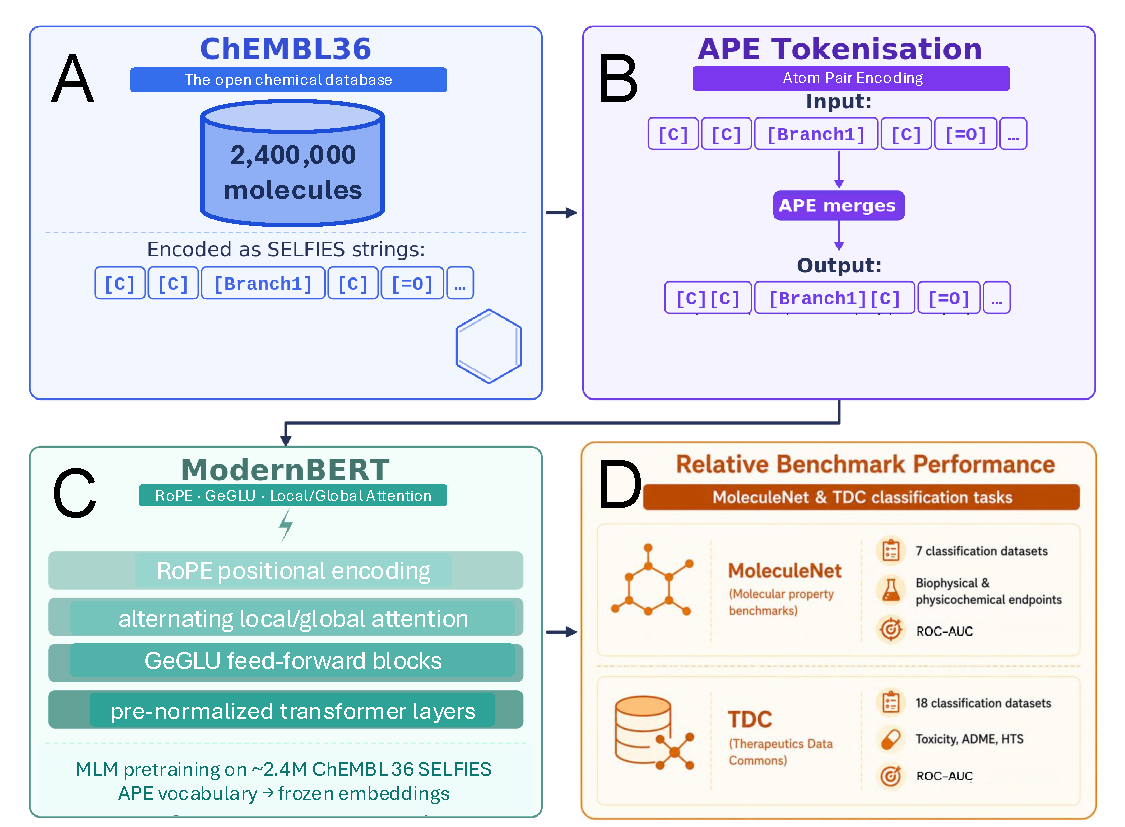
\includegraphics[width=\linewidth]{figures/Fig1_C}
  \caption{%
    \textbf{\model{} pretraining and frozen-evaluation pipeline.}
    Approximately \num{2.4}M unique \chembl{}~36 small molecules are curated,
    canonicalised, and converted to \selfies{} strings, then pre-tokenised with
    the \selfies{}-adapted \ape{} tokeniser (\cref{fig:design}C). A
    \modernbert{} encoder is trained from scratch on this corpus with the masked
    language modelling (MLM) objective, yielding \model{}. For evaluation the
    encoder is \emph{frozen}: mean-pooled final-layer token embeddings over
    non-special \selfies{} tokens are extracted without any gradient updates
    and passed to lightweight downstream classifiers (ridge, random forest,
    $k$-nearest neighbours) on 25 binary molecular property-prediction
    benchmarks, where \model{} is compared against fixed fingerprint and
    pre-trained string-encoder baselines under an identical protocol.
  }%
  \label{fig:overview}
\end{figure}

\begin{figure}[htbp]
  \centering
  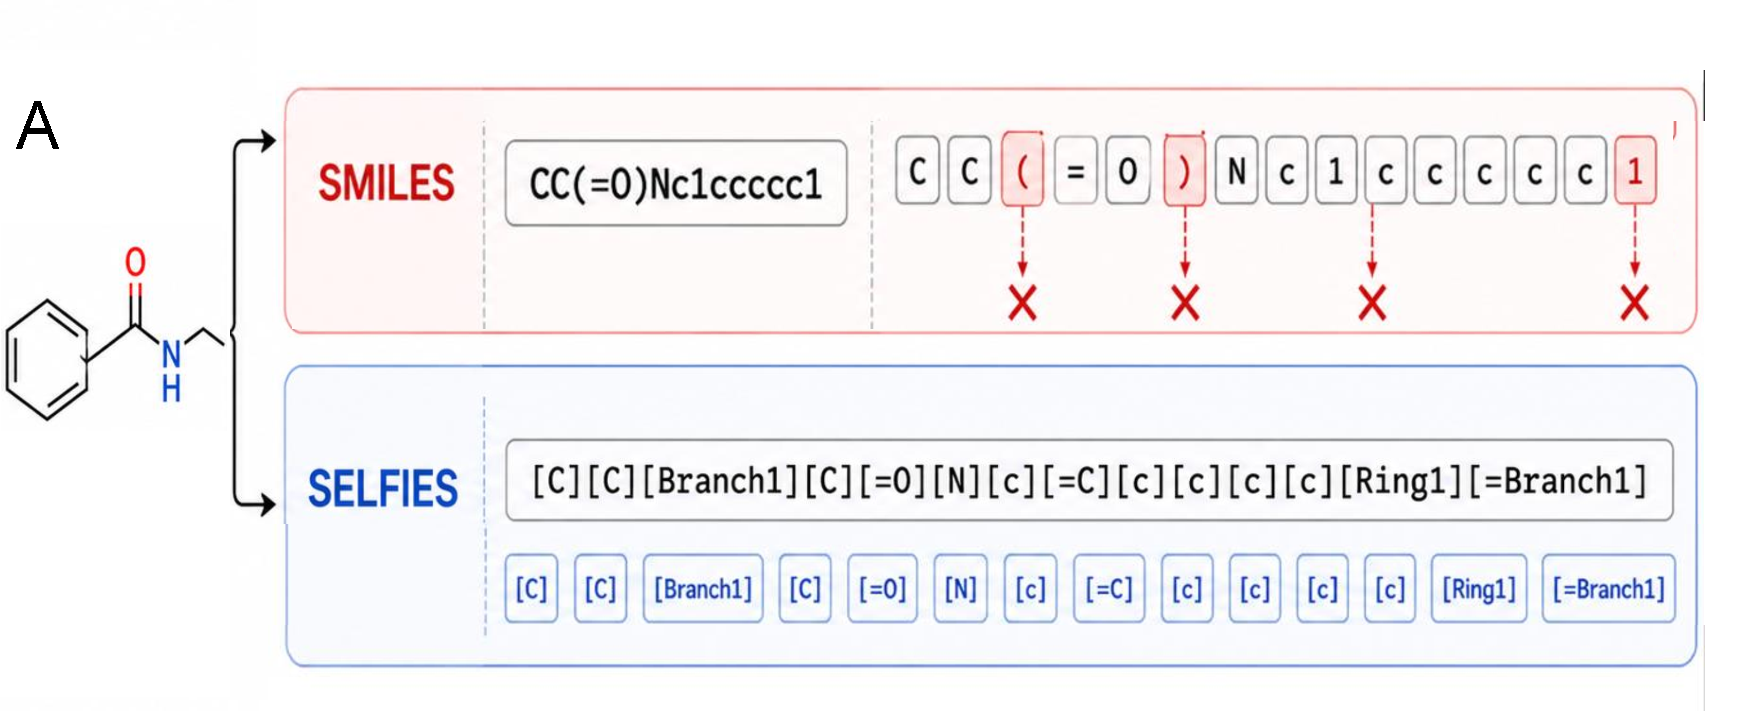
\includegraphics[width=\linewidth]{figures/Fig1_A}\\[0.6em]
  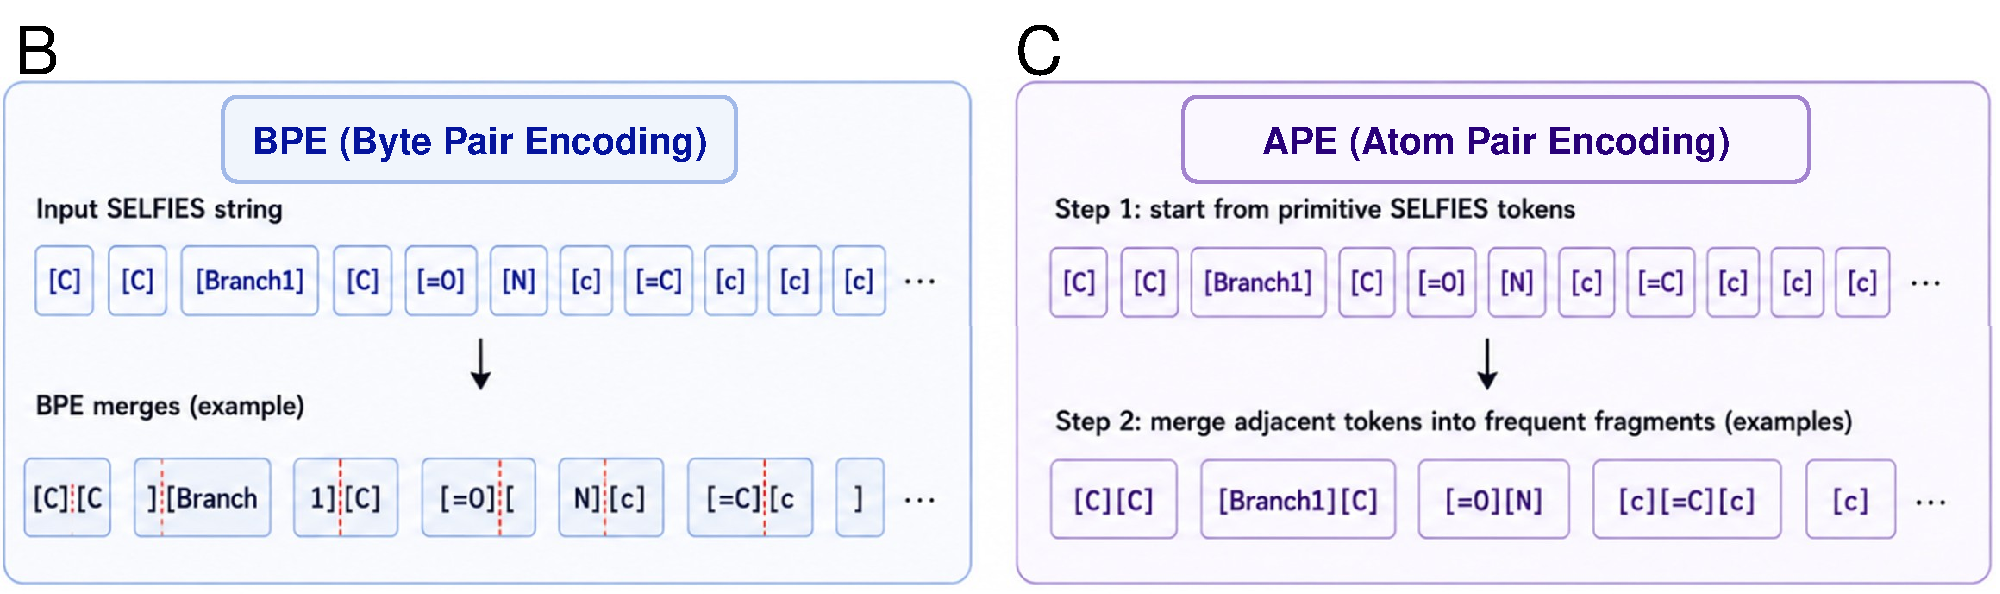
\includegraphics[width=\linewidth]{figures/Fig1_B}
  \caption{%
    \textbf{Method comparison of the two molecular design choices in \model{}:
    input representation and tokenisation.}
    \textbf{(A)}~\emph{Input representation: \smiles{} versus \selfies{}.}
    The same molecule is shown encoded as a \smiles{} string (top) and as a
    \selfies{} string (bottom). \smiles{} tokens can violate chemical syntax
    under perturbation or naive tokenisation --- mismatched brackets and
    ill-formed ring-closure indices are marked with red crosses --- whereas
    every syntactically valid \selfies{} \emph{string} decodes to a
    chemically valid molecule~\citep{krennSELFIESSelfReferencingEmbedded2020}.
    \textbf{(B)}~\emph{Byte Pair Encoding (BPE).}
    BPE merges \selfies{} symbols by raw character frequency without chemical
    awareness, splitting bracketed symbols and producing chemically meaningless
    vocabulary entries (dashed red markers).
    \textbf{(C)}~\emph{Atom Pair Encoding (\ape{}).}
    \ape{} restricts merges to adjacent complete \selfies{} primitives, so every
    vocabulary entry is a valid concatenation of complete \selfies{} symbols
    rather than a character-level artefact~\citep{leonComparingSMILESSELFIES2024}.
  }%
  \label{fig:design}
\end{figure}

% ============================================================
\section{Related Work}%
\label{sec:related-work}
% ============================================================

The introduction motivated the three design choices behind \model{}; this
section places them in the context of prior work along the four axes most
relevant to a frozen \selfies{} embedder --- molecular string representations,
molecular language models, modern encoder architectures, and molecular
tokenisation --- and identifies the specific models we later use as baselines.

\subsection{Molecular String Representations}
\label{sec:rel-representations}

The chemical-validity guarantee of \selfies{} holds under arbitrary mutation:
as reported by \citet{krennSELFIESSelfReferencingEmbedded2020}, a single random
bit-flip leaves a \smiles{} string valid only 26.6\% of the time and ten
bit-flips reduce validity to 0.2\%, whereas \selfies{} remains 100\% valid in
both cases. The representation
is also complete, meaning that every molecule can be encoded, and it can serve as a drop-in
input to any model. In generative settings, VAEs and GANs trained on \selfies{}
populate their latent spaces with two orders of magnitude more diverse valid
molecules than equivalent \smiles{}-based
models~\citep{krennSELFIESSelfReferencingEmbedded2020}.

\subsection{Molecular Language Models}
\label{sec:rel-lms}

The fingerprint ECFP~\citep{rogersExtendedConnectivityFingerprints2010} remains the
dominant deterministic baseline: a circular-substructure fingerprint
with no trainable parameters that continues to compete with learned
representations on many property prediction tasks.
Among learned string encoders, ChemBERTa-2~\citep{ahmadChemBERTa2TowardsChemical2022}
revisited the RoBERTa-on-\smiles{} recipe, pretraining on PubChem
\smiles{} and comparing masked language modelling with multi-task
regression (MTR) over computed RDKit descriptors.
MoLFormer~\citep{rossLargescaleChemicalLanguage2022} scaled the
masked-language-modelling approach to 1.1B molecules and introduced a
linear-attention
transformer, making it the largest-scale \smiles{} string model and
a key large-scale reference point.
SELFormer~\citep{yukselSELFormerMolecularRepresentation2023} is the
closest prior work to \model{}: a RoBERTa encoder pre-trained with MLM
on 2M drug-like \selfies{} strings from \chembl{}.
Several adjacent molecular foundation models use different pretraining
objectives or architectures. Chemformer~\citep{irwinChemformerPretrainedTransformer2022}
uses a sequence-to-sequence transformer for computational chemistry tasks,
whereas CDDD~\citep{winterLearningContinuousDataDriven2019} learns continuous
molecular descriptors by translating between equivalent molecular strings.
Recent encoder-only work such as ChemBERTa-3~\citep{singhChemBERTa3OpenSource2025}
and MolEncoder~\citep{krugerMolEncoderOptimalMasked2025} continues to refine
training recipes for chemical BERT-style models. Recent contrastive and
multimodal approaches such as CLAMP~\citep{seidlEnhancingActivityPrediction2023}
and COATI~\citep{axelrodCOATIMultimodalContrastive2024} extend molecular
embeddings beyond pure string reconstruction by incorporating assay text,
3D information, or other paired supervision. These models broaden the
representation-learning landscape but answer a different question from the
one addressed here: how far a compact, encoder-only \selfies{} MLM can be
pushed as a frozen molecular embedder.
A large and growing literature applies graph neural networks and
graph transformers to molecular representation learning; representative
examples include GROVER~\citep{rongGroverTransformerSelfsupervised2020},
GIN~\citep{huStrategiesPretrainingGraph2020},
GraphMVP~\citep{liuPretrainingMolecularGraph2022},
and Uni-Mol~\citep{zhouUniMolUniversal3D2023}.
These graph-based methods are outside the scope of \model{}, which
operates on sequential \selfies{} strings without explicit graph
structure. Broader benchmarking studies have nevertheless shown that the
relative value of learned molecular representations depends strongly on the
dataset, split strategy, chemical-series structure, and amount of labelled
data available~\citep{yangAnalyzingLearnedMolecular2019,dengSystematicStudyKey2023}.
This motivates treating ECFP4 and other fixed representations as serious
baselines rather than as outdated reference points.

\subsection{Modern BERT Architectures}
\label{sec:rel-modernbert}

\modernbert{}~\citep{warnerSmarterBetterFaster2024} is an encoder-only
transformer that consolidates post-BERT architectural advances into a
production-quality model trained on 2 trillion tokens of text, code, and
scientific literature with a native 8\,192-token context window.
Its key design choices are: Rotary Position Embeddings
(RoPE)~\citep{suRoFormerEnhancedTransformer2023} replacing absolute positional
encodings; \emph{alternating local and global attention}, in which most layers
apply a sliding-window kernel and periodically interleaved layers apply
full-sequence attention, executed with the IO-aware Flash
Attention~\citep{daoFlashAttentionFastMemoryEfficient2022} kernel; GeGLU
feed-forward activations; and unpadded sequence processing, which removes
padding tokens to eliminate wasted compute.
The two released variants for natural language use are \modernbert{}-base (149M parameters) and
\modernbert{}-large (395M). They are trained with a 30\% MLM masking rate and
achieve state-of-the-art results among encoder-only models on natural-language
and code benchmarks.

\subsection{Molecular Tokenisation}
\label{sec:rel-tokenisation}

The atom-preserving \ape{} tokeniser~\citep{leonComparingSMILESSELFIES2024}
(\cref{sec:ape-tokeniser}) was shown to outperform standard BPE in a controlled
comparison of RoBERTa-based models pre-trained on 1M PubChem molecules and
fine-tuned on MoleculeNet, with the largest gains on \selfies{} representations
(ROC-AUC improvements of $+$0.059 on BBBP and HIV and $+$0.017 on Tox21;
Table~6 of \citealt{leonComparingSMILESSELFIES2024}), a result attributed to
its merges aligning with \selfies{}'s symbol-level structure.

% ============================================================
\section{Methods}%
\label{sec:methods}
% ============================================================


\subsection{Atom Pair Encoding Tokeniser}
\label{sec:ape-tokeniser}

We use a custom reimplementation of the \ape{} algorithm
\citep{leonComparingSMILESSELFIES2024,mayuareAPETokenizer} with
several modifications for \selfies{} pretraining at scale, detailed in the
paragraphs below: molecular-aware pre-tokenisation that restricts merges to
complete \selfies{} primitives, frequency- and span-controlled vocabulary
construction, deterministic greedy longest-match inference, and post-training
injection of benchmark-observed primitives.

\paragraph{Molecular-aware pre-tokenisation.}
\selfies{} strings are first split on a regex that isolates each complete
bracket-enclosed primitive, so merges operate only over whole \selfies{}
primitives and every vocabulary entry is a valid concatenation of complete
symbols.

\paragraph{Vocabulary construction.}
Merging is controlled by two criteria: a minimum merge frequency
(\texttt{min\_freq}~$=3000$), which halts merging once the most frequent
adjacent pair co-occurs fewer than 3\,000 times, and a maximum merge span
(\texttt{max\_merge\_pieces}~$=2$), which excludes candidates spanning more
primitives to avoid long, uninformative concatenations. In practice
\texttt{min\_freq} is the binding early-stopping criterion. Full tokeniser
statistics are reported in \cref{tab:tokeniser-stats} (\cref{app:tokeniser}).

\paragraph{Greedy longest-match tokenisation.}
At inference, each position is consumed by the longest matching vocabulary
entry, looking up to \texttt{max\_merge\_pieces} positions ahead. The procedure
is deterministic and $O(n\cdot\texttt{max\_merge\_pieces})$ per sequence, with
an \texttt{<unk>} fallback only when no single primitive is in-vocabulary.

\paragraph{Post-training symbol injection.}
After merge learning but before model pretraining, any valid \selfies{}
primitive that appears $\ge 10$ times in the benchmark molecules but is absent
from the learned vocabulary is appended. This uses only primitive-frequency
information; no benchmark labels or train/test split information are used in
this step. It guarantees a zero unknown-token rate on evaluation molecules; all
model weights were initialised and trained on the completed 631-token vocabulary
from the outset.

\subsection{Model Architecture}
\label{sec:architecture}

Both \model{} variants use the \modernbert{} encoder backbone
(\cref{sec:rel-modernbert})~\citep{warnerSmarterBetterFaster2024} in its default
configuration: RoPE, GeGLU feed-forward blocks, pre-normalisation, no
linear-layer biases. It uses unpadded Flash Attention with global attention
every 3 layers and a 128-token local sliding window. They are trained from
scratch on our \selfies{} \ape{} vocabulary; no weights are transferred from
the official \modernbert{} checkpoints~\citep{warnerModernBERTBlog2024}.
Per-variant hyper-parameters are listed in \cref{tab:model-config}
(\cref{app:training-details}).
\model{}-small (34.1M parameters, 512-dimensional hidden state) sits in the
compact regime below Chemformer~\citep{irwinChemformerPretrainedTransformer2022}
(45M), MoLFormer-XL~\citep{rossLargescaleChemicalLanguage2022} (46.8M), and
Uni-Mol~\citep{zhouUniMolUniversal3D2023} (47.6M), and is notably smaller than
the closest \selfies{} comparator SELFormer (86.7M). \model{}-base (114.3M
parameters, 768-dimensional) is significantly larger than the existing models considered here.

\subsection{Pretraining Data}
\label{sec:pretraining-data}

Pretraining data are sourced from \chembl{}~36~\citep{zdrazilChEMBLDatabase20232024}
via the \texttt{lukaskim/ChEMBL-36} Hugging Face dataset\footnote{\url{https://huggingface.co/datasets/lukaskim/ChEMBL-36}}.
Molecules are deduplicated by \texttt{standard\_inchi\_key}, parsed and
lightly sanitised with RDKit~\citep{landrumRDKitOpenSourceCheminformatics} (ring perception and aromaticity assignment
only, avoiding full sanitisation), and canonicalised to isomeric
canonical \smiles{} using RDKit's \texttt{MolToSmiles} with
\texttt{isomericSmiles=True}.
The resulting canonical \smiles{} strings are then encoded to
\selfies{}~\citep{krennSELFIESSelfReferencingEmbedded2020} using the
\texttt{selfies} Python package.
Molecules that fail RDKit parsing, limited sanitisation,
canonicalisation, or \selfies{} encoding are excluded.
We further filter by size and type, retaining only entries flagged as
small molecules with $3 \le$ heavy atoms $\le 100$ and molecular weight
$\le 1000$\,Da.
Train and validation splits ($99\%$/$1\%$) are assigned deterministically
by SHA-1 hashing of a stable per-molecule identifier (preferring the
standard InChIKey, with fallbacks to ChEMBL~ID, canonical \smiles{}, and
\selfies{} in that order) with seed~13,
yielding \num{2390317} training and \num{24228} validation molecules.
The resulting \selfies{} strings are subsequently pre-tokenised with the
\ape{} tokeniser~\citep{leonComparingSMILESSELFIES2024} using greedy
longest-match tokenisation.
The full curation and pre-tokenisation pipeline is available at
\url{https://github.com/HauserGroup/ModernMolBERT}. The final dataset is available on \url{https://huggingface.co/HauserGroup}.

\subsection{Pretraining Procedure}
\label{sec:pretraining-procedure}

Both \model{} variants are trained from scratch with the masked language
modelling (MLM) objective and no auxiliary tasks. Training runs for 30{,}000
steps at an effective batch size of 256 and a maximum sequence length of 128
tokens. For each variant, the masking rate and peak learning rate are selected
by a $3\times3$ grid search (\cref{sec:ablations}); the remaining optimisation
settings (AdamW, weight decay, gradient clipping, \texttt{bf16}, linear warmup,
and cosine decay) are fixed and reported in \cref{tab:hparams}
(\cref{app:training-details}). Validation loss and masked-token accuracy
converge smoothly within the fixed step budget (\cref{fig:loss-curves}).

\paragraph{Masking strategies.}
We implement three masking strategies as a selectable data-collator component.
\emph{Standard} masking draws an independent Bernoulli mask per eligible token.
\emph{Span} masking masks contiguous spans with lengths drawn from a Geometric
distribution ($p=0.4$, clamped to 6 tokens), following SpanBERT's span
selection but without its Span Boundary
Objective~\citep{joshiSpanBERTImprovingPreTraining2020}.
\emph{Heteroatom-biased span} masking up-weights span-start positions at \ape{}
tokens containing a heteroatom primitive (N, O, S, P, F, Cl, Br, I, Se, Si),
identified by a bracket-aware \selfies{} regex; spans extend beyond the start,
so masking is enriched around rather than restricted to these tokens. It is a
parser-free proxy for the functional-group masking of
\citet{pengPretrainedMolecularLanguage2025}, using the \ape{} bracket
vocabulary in place of explicit SMARTS matching. All three apply the standard
BERT corruption rule (80\% \texttt{[MASK]}, 10\% random token, 10\% unchanged).
The released models use standard masking; \cref{sec:ablations} compares all
three.

\subsection{Evaluation Protocol}
\label{sec:eval-protocol}

All benchmark tasks are evaluated using frozen \model{} embeddings, following
the lightweight protocol of \citet{praskiBenchmarkingPretrainedMolecular2025}.\footnote{%
Using their public benchmark code at
\url{https://github.com/MLCIL/benchmarking_molecular_models}.}
For each molecule, the encoder is run in inference mode and molecule-level
representations are obtained by mean-pooling the final-layer token embeddings
over non-special \selfies{} tokens; no model parameters are updated. These
embeddings are evaluated with three lightweight downstream models chosen to
span complementary inductive biases --- a linear ridge classifier, ensemble
random forests, and instance-based $k$-nearest neighbours --- so that
representation quality is not judged through a single decision boundary. We
adopt these three heads, and their cross-validation search grids, directly from
the benchmark protocol of \citet{praskiBenchmarkingPretrainedMolecular2025} to
keep the comparison with their reported baselines exact; hyperparameters are
selected by cross-validation on the training split, with performance reported
on the held-out test split. All tasks are scored by ROC-AUC. For multi-task
datasets, missing endpoint labels are treated as unmeasured: downstream
classifiers are fit endpoint-wise on finite labels (in both cross-validation
and test evaluation), and dataset-level ROC-AUC is averaged over endpoints with
finite labels and both classes present in the test split. The best downstream
model per dataset is used in the main comparison.

% ============================================================
\section{Experiments}%
\label{sec:experiments}
% ============================================================


\subsection{Benchmark Datasets}
\label{sec:benchmarks}

We evaluate on 25 binary classification datasets drawn from two
sources: 18 datasets from the Therapeutics Data
Commons~(TDC)~\citep{huangTherapeuticsDataCommons}, spanning toxicity
(4 datasets), ADME (12 datasets), and high-throughput screening (2
datasets); and 7 datasets from
MoleculeNet~\citep{wuMoleculeNetBenchmarkMolecular2018}, covering a
range of biophysical and physical chemistry endpoints.
Dataset sizes range from 475 to 93\,087 compounds, with task counts
ranging from 1 to 27 (SIDER).
The full list with per-dataset statistics is given in Table~4 of
\citet{praskiBenchmarkingPretrainedMolecular2025}, whose benchmark
selection we follow directly.
All datasets are evaluated by ROC-AUC.

\subsection{Baselines}
\label{sec:baselines}

We compare \model{} against both fixed and learned molecular representations.
ECFP4 is the classical non-neural baseline~\citep{rogersExtendedConnectivityFingerprints2010,yangAnalyzingLearnedMolecular2019,dengSystematicStudyKey2023}.
The pre-trained string-model baselines each isolate one axis of comparison:
ChemBERTa-2 is the closest-scale RoBERTa-style \smiles{} MLM; SELFormer
isolates the use of \selfies{} with a BERT/RoBERTa-era encoder; and
MoLFormer\footnote{MoLFormer's inference relies on the ONNX Runtime for its
linear-attention kernel, which has limited compatibility with Python newer than
$\approx$3.10; embedding extraction therefore required a pinned legacy
environment.} is a large-scale \smiles{} reference trained on substantially
broader PubChem and ZINC data.
Because \model{} is trained purely with MLM, we use the MLM-trained variant of
each baseline so that the comparison is not confounded by the pretraining
objective: SELFormer and MoLFormer are
MLM-pre-trained~\citep{yukselSELFormerMolecularRepresentation2023,rossLargescaleChemicalLanguage2022},
and for ChemBERTa-2 we use the MLM checkpoint
(\texttt{seyonec/ChemBERTa-77M-MLM}) rather than the multi-task-regression
variant~\citep{ahmadChemBERTa2TowardsChemical2022}. Auxiliary-objective and
multi-task-regression pretraining therefore falls outside this MLM-only
comparison. No model, including \model{}, is fine-tuned end-to-end; all neural
baselines are evaluated as frozen embedders under the same downstream protocol.

% ============================================================
\section{Results}%
\label{sec:results}
% ============================================================


\subsection{\model{} Approaches Fingerprints and Improves on Closest-Scale String Encoders}
\label{sec:main-results}

The main comparison aggregates ROC-AUC across the 25 binary classification
benchmark datasets described in \cref{sec:benchmarks}. For each
representation--dataset pair, we report the best cross-validated downstream
estimator among ridge classification, random forests, and $k$-nearest
neighbours, following the frozen mean-pooled embedding protocol in
\cref{sec:eval-protocol}.
For multi-endpoint datasets, endpoint ROC-AUCs are averaged before aggregation.
This presentation separates the quality of the pre-trained representation from
gains attributable to end-to-end fine-tuning, and therefore directly tests
whether \model{} provides useful off-the-shelf molecular embeddings.
Throughout, ROC-AUC values are reported $\times100$, so one point corresponds
to $0.01$ ROC-AUC. Direct paired comparisons
use only jointly evaluated datasets, reported in \cref{fig:bootstrap-ci} and
\cref{tab:bootstrap-cis}.
\Cref{tab:main-results} reports mean ROC-AUC by task group; per-dataset
results for all models are given in \cref{tab:pertask}.

\begin{figure}[htbp]
  \centering
  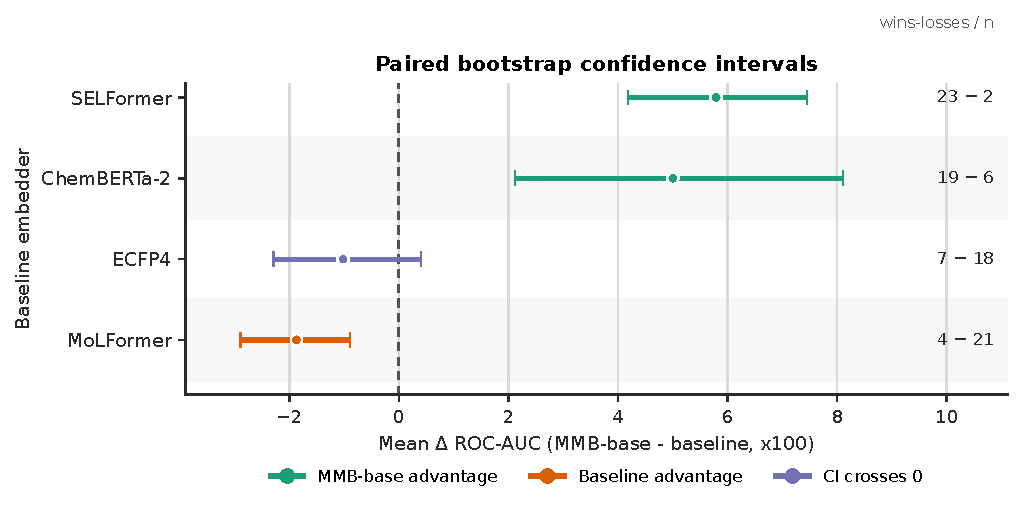
\includegraphics[width=0.82\linewidth]{figures/bootstrap_ci_forest}
  \caption{%
    \textbf{Paired bootstrap confidence intervals for \model{}-base
    vs.\ each baseline ($n = 23$ jointly evaluated datasets).}
    Each row shows the mean $\Delta$ ROC-AUC ($\times$100) between
    \model{}-base and one baseline (positive = \model{}-base higher),
    with 95\% bootstrap confidence intervals ($B = 10{,}000$ resamples)
    and the number of datasets on which \model{}-base scores higher.
    The dashed line marks zero. The intervals for SELFormer and ChemBERTa-2
    lie entirely above zero, that for MoLFormer entirely below, and that for
    ECFP4 spans zero. Numerical values are given in \cref{tab:bootstrap-cis}
    and full per-dataset results in \cref{tab:pertask}.
  }%
  \label{fig:bootstrap-ci}
\end{figure}

\begin{table}[htbp]
  \centering
  \small
  \begin{tabularx}{\linewidth}{l r r r r r}
    \toprule
    \textbf{Model} & \textbf{TDC-ADME} & \textbf{TDC-Tox} & \textbf{TDC-HTS} & \textbf{MoleculeNet} & \textbf{Overall} \\
    \midrule
    ECFP4 & 81.1 & 85.0 & \textbf{68.6} & 74.8 & 78.9 \\
    ChemBERTa-2 (MLM) & 77.3 & 73.1 & 66.3 & 67.2 & 72.9 \\
    SELFormer & 75.1 & 74.6 & 61.1 & 68.8 & 72.1 \\
    MoLFormer & \textbf{81.5} & \textbf{85.2} & 66.8 & \textbf{77.6} & \textbf{79.8} \\
    \midrule
    \textbf{\model{}-small} & 79.6 & 83.7 & 64.8 & 73.7 & 77.4 \\
    \textbf{\model{}-base} & 80.7 & 83.8 & 64.4 & 73.7 & 77.9 \\
    \bottomrule
  \end{tabularx}
  \caption{%
    Mean ROC-AUC ($\times100$) on the 25-dataset benchmark of \citet{praskiBenchmarkingPretrainedMolecular2025}, broken down by
    task group. Each entry averages per-dataset ROC-AUC using the best cross-validated downstream head (ridge / random forest / $k$NN);
    for multi-endpoint datasets, endpoint scores are averaged before aggregation.
    \emph{Overall} is the unweighted mean across all 25 benchmark datasets.
    \textbf{Bold} marks the best value per column.
  }%
  \label{tab:main-results}
\end{table}


\model{}-base attains a mean ROC-AUC of 77.4 across 24 evaluated benchmark
datasets (Tox21 is omitted for \model{}-base; see \cref{tab:pertask}), and
\model{}-small attains 77.3 across all 25 datasets
(per-dataset results in \cref{tab:pertask}). For comparison, ECFP4 reaches 78.9, MoLFormer
79.8, ChemBERTa-2 72.9, and SELFormer 72.1. Both \model{} variants therefore
land between the strong fixed-fingerprint and large-scale \smiles{} baselines
(ECFP4, MoLFormer) and the closest-scale pre-trained string encoders
(ChemBERTa-2, SELFormer), which they exceed by roughly four to five ROC-AUC
points. \Cref{fig:baseline-paired} shows the corresponding per-dataset paired
comparisons against each baseline.

By task group, \model{} is strongest on the property-driven TDC tasks: it is
competitive with ECFP4 on ADME (\model{}-base 80.7 vs.\ 81.1) and toxicity
(83.8 vs.\ 85.0), the endpoints most closely tied to physicochemical structure
(\cref{fig:group-bars}). Its weakest group is the two-task TDC-HTS set (64.4),
where all neural embedders trail ECFP4. On MoleculeNet, MoLFormer shows its
clearest advantage (77.6 vs.\ \model{}-base 70.7), consistent with its much
larger and more chemically diverse pretraining corpus. This pattern is
consistent with frozen learned embeddings transferring best to tasks governed by
global physicochemical character rather than rare substructure recognition, an
interpretation in line with broader analyses of when learned molecular
representations help~\citep{yangAnalyzingLearnedMolecular2019,dengSystematicStudyKey2023}.

Relative to ECFP4, \model{} approaches but does not surpass the fingerprint
baseline. \model{}-base exceeds ECFP4 on 7 of the 23 jointly evaluated datasets,
with a mean $\Delta$ ROC-AUC of $-1.0$ and a 95\% bootstrap confidence
interval of $[-2.5,\;+0.5]$ (\cref{tab:bootstrap-cis}); the interval
spans zero, consistent with neither a reliable advantage nor a reliable
deficit at this scale. \model{}-small wins on 5 of 25. As such,
\model{} is approaching, rather than surpassing, ECFP4 under the frozen-embedding
protocol, consistent with the continued strength of circular fingerprints in
low-data property prediction.

The comparison most diagnostic of \model{}'s design is SELFormer, the closest
prior \selfies{} encoder (a RoBERTa-era backbone on the same representation).
Here \model{} improves clearly and consistently: \model{}-base exceeds
SELFormer on 21 of 23 jointly evaluated datasets (mean $\Delta$ ROC-AUC
$+5.4$; 95\% CI $[+3.9,\;+7.1]$; \cref{tab:bootstrap-cis}), and
\model{}-small on 24 of 25. Because both models consume \selfies{} inputs, this
gap is consistent with the combined benefit of \modernbert{}-era architectural
choices, \ape{} tokenisation, and differences in the training recipe; matched
single-axis ablations would be required to assign the gain to individual
components. \model{} likewise exceeds the \smiles{}-based ChemBERTa-2 by 4.6
points on 23 jointly evaluated datasets (mean $\Delta$ $+4.6$; 95\% CI
$[+1.6,\;+7.9]$). It does not reach MoLFormer, which is pre-trained on roughly
$400\times$ more molecules (mean $\Delta$ $-1.7$; 95\% CI $[-2.6,\;-0.7]$).

A qualitative view of the learned representation is given in
\cref{fig:embedding-space}: PaCMAP projections of the frozen \model{}-base
embeddings organise molecules along smooth, chemically interpretable gradients
in physicochemical descriptors spanning both whole-molecule properties
(lipophilicity, drug-likeness, polarity, size) and more local structural counts
(flexibility, aromaticity), indicating that the embedding space encodes
chemically meaningful structure even though it is never given these properties
as training signal. We read this only qualitatively: the smooth arrangement
shows that neighbouring embeddings tend to correspond to chemically similar
molecules, which is the property that makes the embeddings useful for the
similarity-driven downstream heads above, and we draw no quantitative
conclusions from the projected coordinates themselves.

\begin{figure}[htbp]
  \centering
  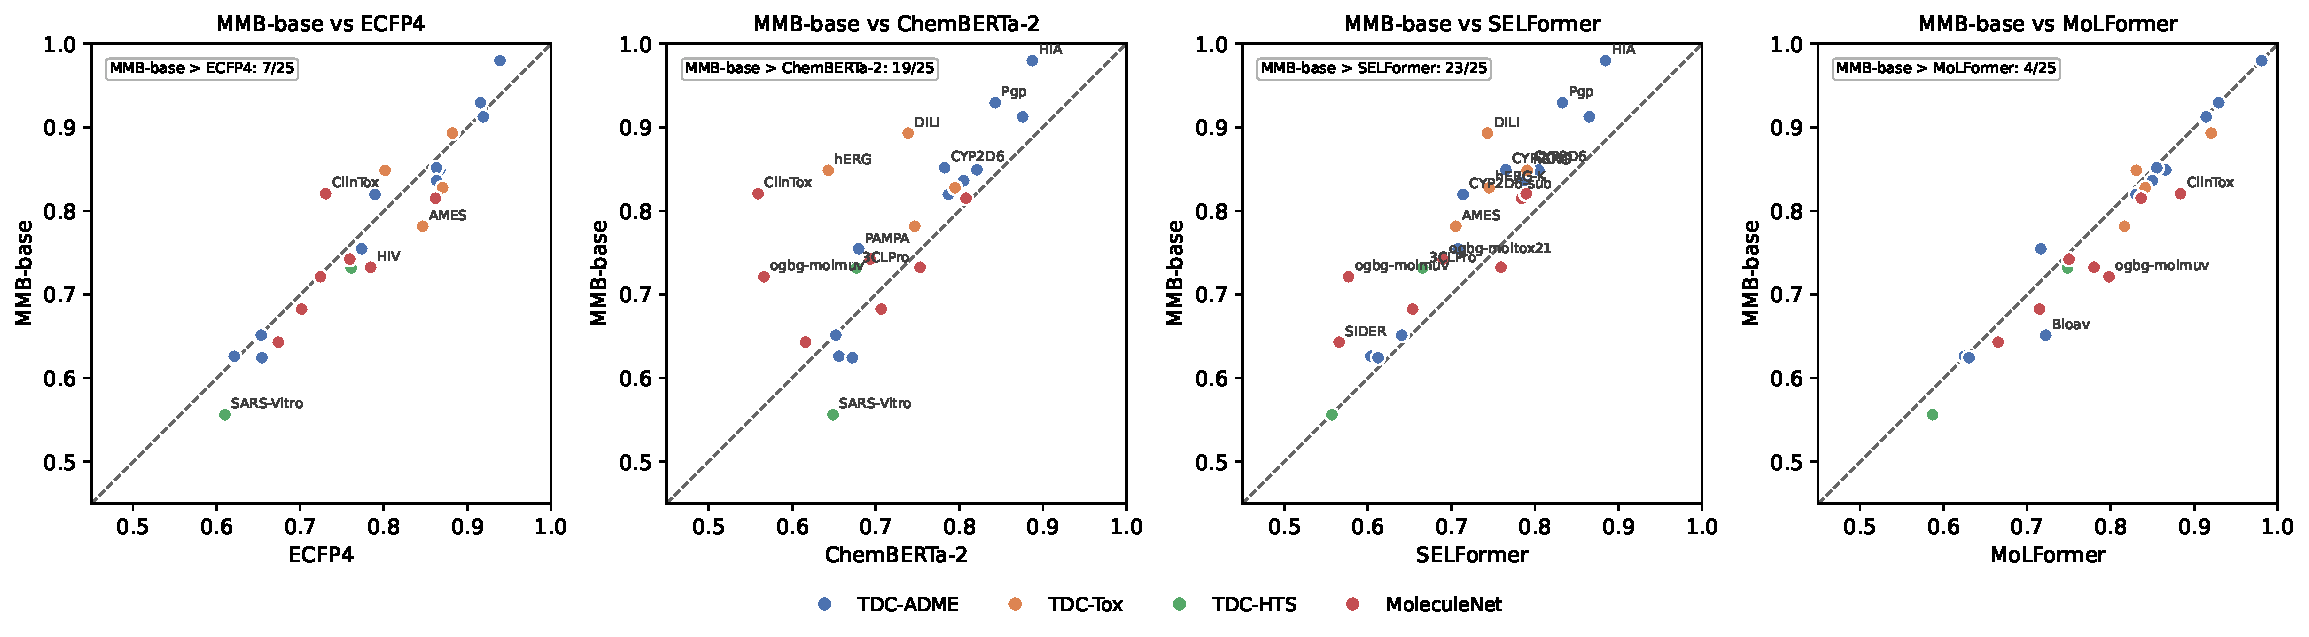
\includegraphics[width=\linewidth]{figures/Fig_baselines}
  \caption{%
    \textbf{Per-task comparison of \model{}-base against the four baseline
    embedders.}
    Each panel is a paired scatter of held-out test ROC-AUC across the
    benchmark tasks (one point per task, best cross-validated downstream head
    per task), with \model{}-base on the $y$-axis and one baseline on the
    $x$-axis: ECFP4, ChemBERTa-2 (MLM), SELFormer, and MoLFormer.
    The dashed line is the identity $y=x$; points above it indicate tasks where
    \model{}-base scores higher. Points are coloured by task group (TDC-ADME,
    TDC-Tox, TDC-HTS, MoleculeNet), tasks with a gap $>0.05$ ROC-AUC are
    labelled, and each inset gives the number of tasks on which \model{}-base
    wins. All encoders are evaluated as frozen embedders under an identical
    protocol; Tox21 is omitted for \model{}-base (\cref{tab:pertask}).
  }%
  \label{fig:baseline-paired}
\end{figure}

\begin{figure}[htbp]
  \centering
  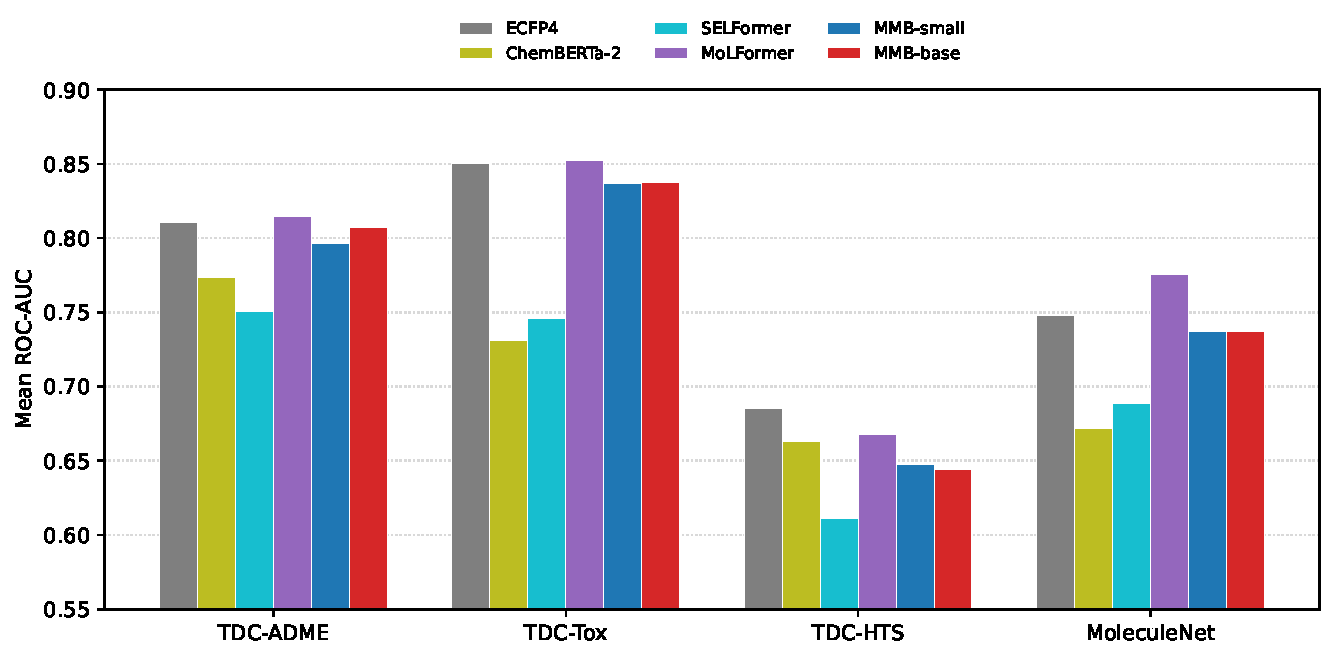
\includegraphics[width=0.85\linewidth]{figures/Fig_groupbars}
  \caption{%
    \textbf{Mean test ROC-AUC by task group.}
    Unweighted mean held-out ROC-AUC within each of the four task groups
    (TDC-ADME, 12 tasks; TDC-Tox, 4; TDC-HTS, 2; MoleculeNet, 7) for ECFP4,
    ChemBERTa-2 (MLM), SELFormer, MoLFormer, and the two released \model{}
    variants, all evaluated as frozen embedders. Group means for the
    masking-strategy ablation variants are omitted here for clarity and reported
    in \cref{tab:pertask}.
  }%
  \label{fig:group-bars}
\end{figure}

\begin{figure}[htbp]
  \centering
  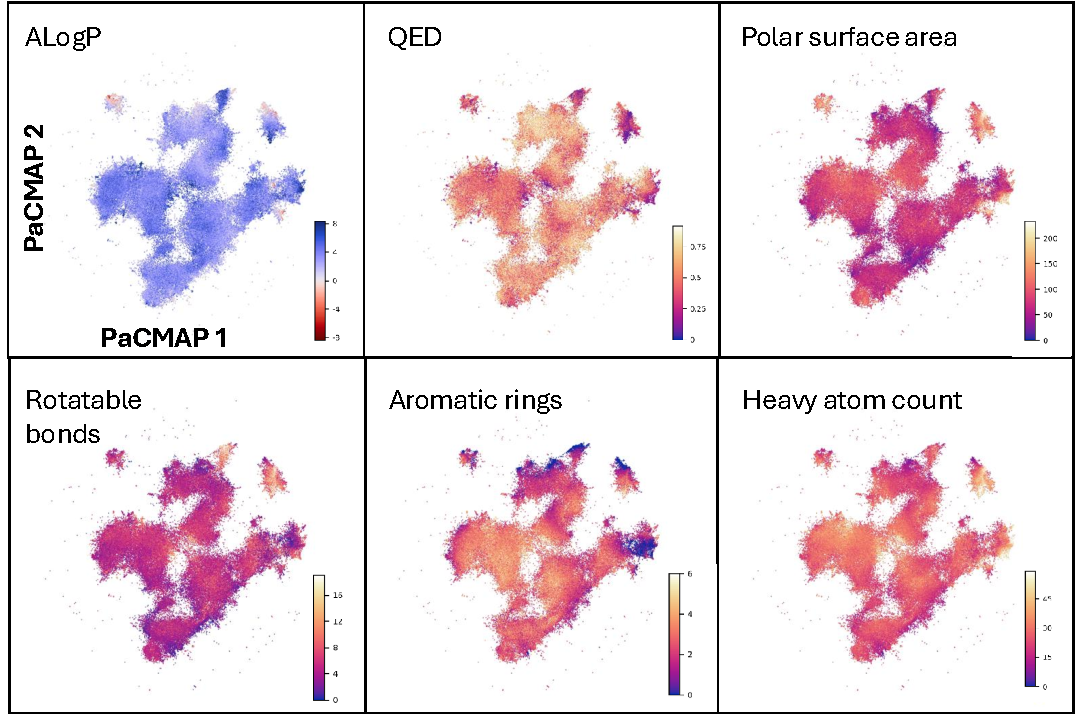
\includegraphics[width=\linewidth]{figures/Fig_4}
  \caption{%
    \textbf{Chemical property gradients across the \model{} embedding space.}
    PaCMAP projection~\citep{wangUnderstandingHowDimension} of frozen
    \model{} molecular embeddings, coloured by selected physicochemical
    properties from \chembl{}~36.
    Each point represents one molecule; colour indicates the corresponding
    property value: ALogP, the quantitative estimate of drug-likeness (QED),
    polar surface area, rotatable bonds, aromatic rings, and heavy atom count.
    PaCMAP is used solely for two-dimensional visualisation of the
    high-dimensional embeddings; the absolute axis coordinates are not
    chemically meaningful, and only relative neighbourhoods and broad spatial
    trends should be interpreted.
  }%
  \label{fig:embedding-space}
\end{figure}

\subsection{Ablation Studies}
\label{sec:ablations}

We ablate two pretraining axes --- the MLM masking strategy and model size ---
on validation MLM metrics (\cref{fig:masking-sweep}; full heatmaps in
\cref{fig:masking-heatmap}) and on downstream ROC-AUC (\cref{fig:four-model}).
The three design choices shared by all released models (the \selfies{}
representation, the \ape{} tokeniser, and the \modernbert{} backbone) are not
isolated here by matched single-axis ablations; they are instead probed jointly
through the external baselines of \cref{sec:main-results}. The
SELFormer comparison, which shares the \selfies{} representation and
dedicated tokeniser and representation ablations are left for future work.

On the validation MLM objective, the choices separate more clearly: for the small model,
span masking at $2\!\times\!10^{-4}$ is strongest and heteroatom-biased span
masking consistently weakest; for the base model, $2\!\times\!10^{-4}$ and
$4\!\times\!10^{-4}$ behave similarly while $8\!\times\!10^{-4}$ diverges. These
differences largely do not carry through to downstream property prediction:
relative to the released small model, the small-to-base size increase changes
mean ROC-AUC by $+0.1$ point (across 24 jointly evaluated datasets), span masking
by $+0.1$ (23 datasets), and heteroatom-biased span masking by $-0.7$
(22 datasets), all within the dataset-to-dataset scatter. The heteroatom-biased deficit is a genuine negative
result: enriching masking around heteroatom tokens is insufficient to improve
frozen embeddings, suggesting the gap to the explicit functional-group masking
of \citet{pengPretrainedMolecularLanguage2025} matters in practice.

Frozen-embedding quality is therefore largely insensitive to masking strategy
and to the small-to-base size increase. This supports releasing the simplest
configuration (standard masking) as the default and is consistent with the
larger gains over SELFormer (\cref{sec:main-results}) arising from the design
choices shared by all released models. The corresponding per-task paired
scatters isolating each pretraining axis are provided in
\cref{fig:four-model} (\cref{app:additional-results}).

\begin{figure}[htbp]
  \centering
  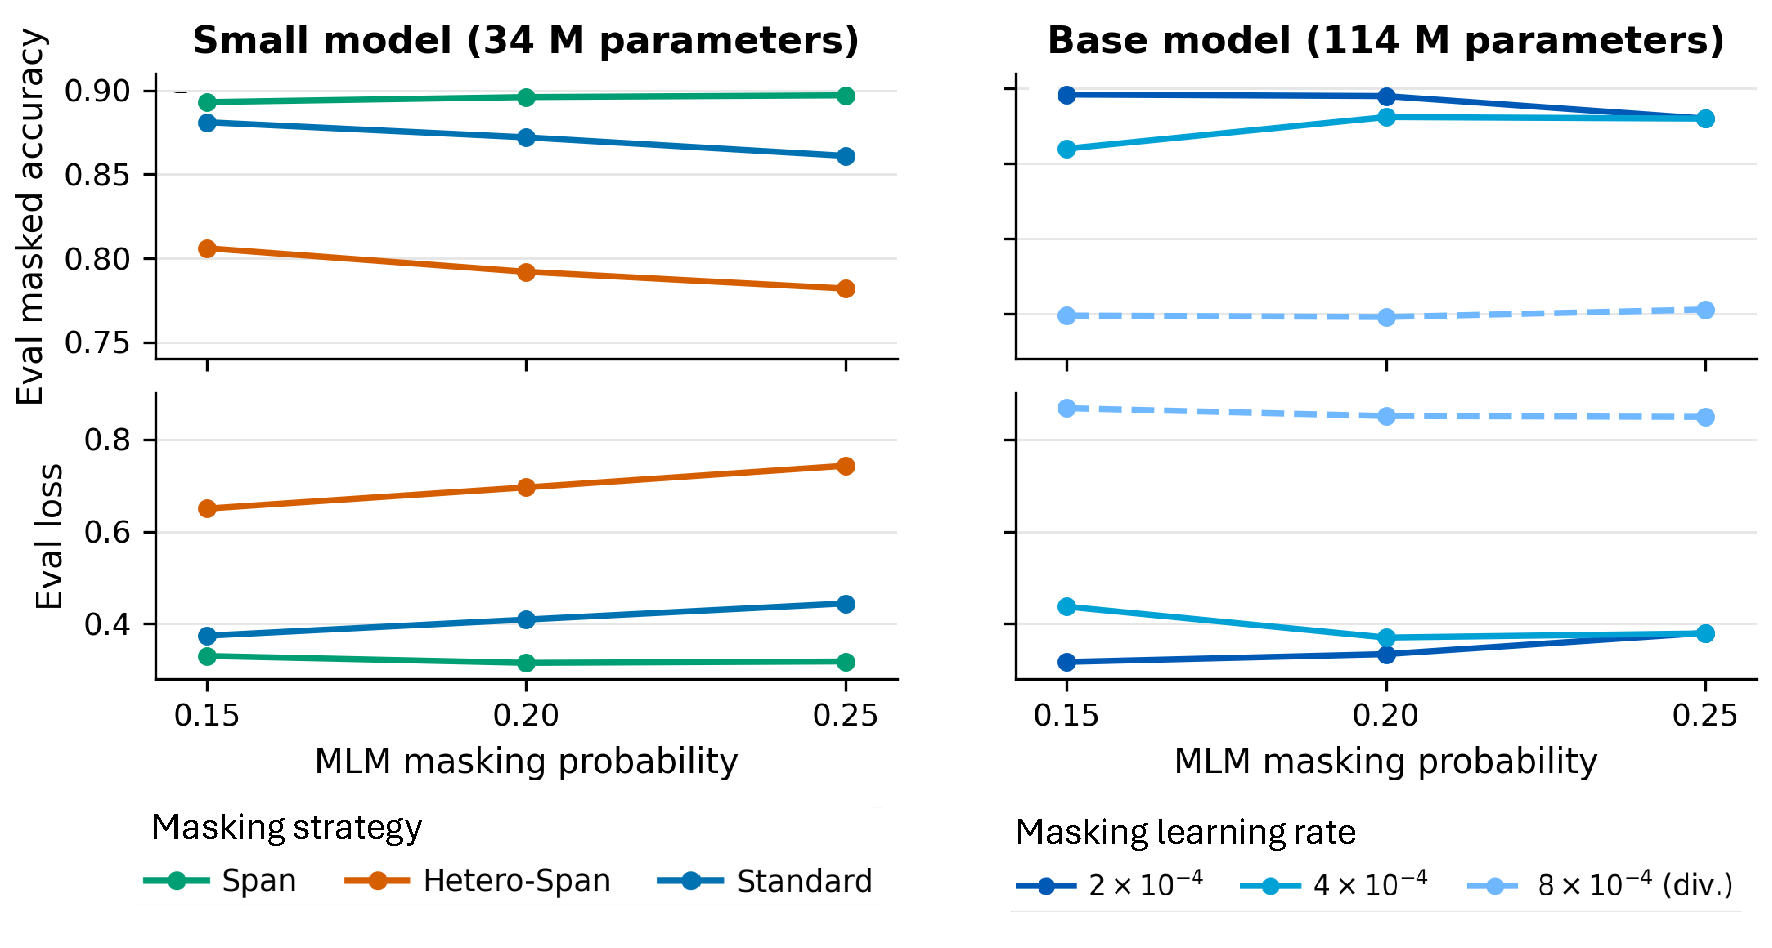
\includegraphics[width=\linewidth]{figures/Fig_3}
  \caption{%
    \textbf{Primary sweep of MLM masking probability, masking strategy, and
    learning rate.}
    Validation performance across MLM masking probabilities for the small
    \model{} ($\sim$34\,M parameters) and base \model{} ($\sim$114\,M
    parameters) models.
    \textbf{(a,b)}~evaluation masked accuracy (higher is better);
    \textbf{(c,d)}~evaluation loss (lower is better); the $x$-axis is the MLM
    masking probability throughout.
    For the small model, line colour denotes masking strategy (span,
    hetero-span, standard); for the base model, all runs use standard masking
    and line colour denotes peak learning rate
    ($2\!\times\!10^{-4}$, $4\!\times\!10^{-4}$, $8\!\times\!10^{-4}$).
    Shaded bands give the min--max range across runs and the asterisk marks the
    run that diverged during training.
    Full heatmaps across all conditions are provided in
    \cref{fig:masking-heatmap}.
  }%
  \label{fig:masking-sweep}
\end{figure}

% ============================================================
\section{Discussion}%
\label{sec:discussion}
% ============================================================

\subsection{Scope and interpretation}
\label{sec:scope}

\model{} is designed around a narrow but practical question: whether a
compact encoder-only model can provide useful frozen molecular embeddings
when trained on chemically valid \selfies{} strings with a \selfies{}-aware
\ape{} tokeniser. This scope differs from large generative chemical language models,
multimodal assay--molecule models, and graph or 3D molecular encoders. The
resulting comparison is therefore most informative when interpreted as a test
of frozen, string-based molecular representation learning rather than as a
claim about all molecular foundation models. \model{} is used here purely as an
encoder, not as a generative model; we therefore do not sample or reconstruct
molecules from it. We note, however, that because both inputs and the MLM head
operate over the \selfies{} vocabulary, any \selfies{} sequence the model
predicts decodes to a chemically valid molecule by construction, so a
generative use of the architecture would inherit \selfies{}' validity guarantee
--- a direction we leave to future work.

Every number in this paper should be read as a \emph{frozen-embedding}
result. No encoder is fine-tuned downstream; each produces a fixed mean-pooled
embedding that is passed to lightweight classifiers. This protocol isolates
representation transferability and mirrors fingerprint-based workflows, where
fixed molecular features are precomputed once and reused across many endpoints.
The fine-tuned behaviour of \model{} is left to future work
(\cref{sec:future-work}).

\subsection{Advances over prior string models}
\label{sec:advances}

Within this frozen-feature setting, the clearest advance is over the closest
prior \selfies{} encoder: holding the molecular representation fixed, \model{}
improves on SELFormer by roughly five ROC-AUC points and is similarly ahead of
the closest-scale \smiles{} MLM, ChemBERTa-2 (\cref{sec:main-results}). Because
the SELFormer comparison shares the \selfies{} representation, this gain is
consistent with benefits from the \modernbert{} backbone and \ape{} tokeniser,
though matched single-axis ablations would be required to isolate each
component's contribution. We do not overstate the result: \model{} is
competitive with, but does not surpass, the strong ECFP4 fingerprint baseline
and trails MoLFormer, which is pre-trained on roughly $400\times$ more
molecules~\citep{rossLargescaleChemicalLanguage2022}. The contribution is
therefore a compact, reproducible
\selfies{} encoder that approaches fixed-fingerprint quality while substantially
improving on prior string-based language models at comparable scale. 

A practical advantage of \model{} is accessibility. ModernMolBERT is released in the standard Hugging Face Transformers format and can be used with the current Python ecosystem without model-specific runtime dependencies, legacy Python versions, custom inference kernels, or external chemistry toolkits at embedding time once inputs are provided as SELFIES strings. Frozen embeddings can therefore be extracted with a few lines of standard Transformers code, making the model easier to incorporate into existing screening, retrieval, and benchmark pipelines than models requiring specialised environments. Likewise, the standalone tokeniser is straightforward to use in a similar fashion.

ModernMolBERT therefore occupies a practical trade-off point rather than a pure performance extreme. Larger or more specialised models remain preferable when maximum benchmark accuracy is the only objective, but many molecular-embedding workflows require representations that are adequate, reproducible, compact, and easy to deploy. In this setting, ModernMolBERT is a reasonable default: it approaches ECFP4, improves over comparable pretrained string encoders, and exposes frozen embeddings through the standard Hugging Face Transformers interface without specialised inference infrastructure.

\subsection{Limitations}
\label{sec:limitations}


\model{} is pre-trained exclusively on \chembl{}~36, a corpus
dominated by drug-like, Lipinski-compliant compounds.
Compared with MoLFormer, which draws from 1.1B PubChem~\citep{kimPubChem2023Update2023} and ZINC~\citep{irwinZINC20FreeUltralargeScale2020}
molecules, \model{}'s training distribution is narrower; generalisation to
natural products, agrochemicals, peptides, macrocycles, or other
under-represented chemical spaces may be limited.
Pretraining uses canonical-\smiles{}-derived \selfies{} strings only;
we do not apply randomised \smiles{} augmentation or multiple-enumeration
strategies, which have been explored as a means of improving representation
diversity in prior molecular language
models~\citep{winterLearningContinuousDataDriven2019,leeSimSonSimpleContrastive2025}.
Like all sequential string models, \model{} has no access to explicit
3D conformational information; graph- and geometry-based models such
as Uni-Mol~\citep{zhouUniMolUniversal3D2023} and
GEM~\citep{fangGeometryenhancedMolecularRepresentation2022} address
this at the cost of greater architectural complexity.
The \selfies{}-adapted \ape{} tokeniser forms merge candidates from
sequence-adjacent \selfies{} primitives rather than reconstructing
the molecular graph; merge boundaries therefore do not necessarily
align with graph-level bond adjacency.
Our evaluation is restricted to binary classification tasks scored
by ROC-AUC, following the benchmark of
\citet{praskiBenchmarkingPretrainedMolecular2025}; performance on
regression tasks, generative objectives, or out-of-distribution
scaffolds is not assessed here.
A further caveat concerns possible train--benchmark overlap: both the
\chembl{}~36 pretraining corpus and several of the benchmark datasets are
derived from overlapping medicinal-chemistry sources, and we do not explicitly
deduplicate benchmark structures against the pretraining set. Some benchmark
molecules or close analogues may therefore also appear during pretraining,
which could modestly inflate absolute scores for all pretrained encoders
evaluated here; the relative comparisons between encoders are less affected,
since every pretrained baseline is exposed to similar public chemical space.
Finally, all models are evaluated as frozen encoders, which may not
reflect relative performance under full fine-tuning; frozen evaluation
may favour representations with broader but shallower chemical
coverage. More generally, systematic comparisons of molecular property
prediction models show that representation learning gains are highly
context-dependent and are affected by data regime, split strategy, and
activity cliffs~\citep{yangAnalyzingLearnedMolecular2019,dengSystematicStudyKey2023}.
These considerations are especially relevant for frozen-feature evaluations,
where the representation must transfer without task-specific adaptation.

\subsection{Future Work}
\label{sec:future-work}

Several extensions follow naturally from the present design, all within the
MLM-only, string-encoder scope of this work. The most direct is broader
pretraining beyond \chembl{}, including PubChem, ZINC, Enamine, or other
sources that better cover natural products, fragments, reagents, and
non-drug-like chemistry. Pretraining \model{} on the same corpora used by the
baselines---for example the PubChem/ZINC mixture behind MoLFormer---would
further allow the architecture and tokeniser to be compared at matched data,
separating the contribution of pretraining scale from that of model design. A
closely related question is how \model{} scales: the present study fixes a
compact small/base pair and a 30{,}000-step budget, and systematically
increasing model size, corpus size, and training compute would establish
whether the remaining gap to large-scale \smiles{} models such as MoLFormer
narrows with scale. A second direction is matched single-axis ablations
of the tokeniser and backbone choices---substituting \ape{} with standard BPE
or the \modernbert{} backbone with a RoBERTa-era encoder---to isolate each
component's contribution to the gains over SELFormer. A third is to explore
\selfies{} encoders as molecular indexing models for chemical search, analogue
retrieval, and dataset auditing, where deterministic valid string encodings and
compact frozen embeddings are operationally attractive.

% ============================================================
\section{Conclusion}%
\label{sec:conclusion}
% ============================================================

We presented \model{}, a family of compact encoder-only transformer models
for \selfies{} molecular language modelling. The models combine the
\modernbert{} encoder architecture with a \selfies{}-adapted \ape{} tokeniser
and are pre-trained from scratch on a curated \chembl{}~36 corpus using the
masked language modelling objective.

On 24 completed benchmark datasets evaluated under the frozen embedding
protocol, \model{}-base achieves a mean ROC-AUC of 77.4. This is competitive
with the strong ECFP4 fingerprint baseline (78.9) and trails the much larger
MoLFormer (79.8), while clearly exceeding the closest prior \selfies{} and
\smiles{} string encoders, SELFormer (72.1) and ChemBERTa-2 (72.9), by four
to five ROC-AUC points. Internal ablations further show that downstream
embedding quality is largely insensitive to masking strategy and to the
small-to-base size increase, so the gains over prior string models are
consistent with the shared \selfies{}, \ape{}, and \modernbert{} design choices.
These results suggest that a modern \selfies{} encoder with an atom-preserving
\ape{} tokeniser can approach fingerprint-level frozen-feature performance while substantially
improving on earlier string-based language models at comparable scale.

The central motivation is practical: molecular string encoders should be
valid by construction, tokenised in chemically meaningful units, and built on
modern efficient transformer components rather than inherited BERT-era
backbones. By evaluating \model{} as a frozen embedder against ECFP4 and
representative pre-trained molecular language models, we position
\selfies{}-based ModernBERT encoders as a reproducible and computationally
manageable foundation for molecular representation learning.


% ============================================================
\section*{Data and Code Availability}
% ============================================================

Training code and evaluation scripts are available at
\url{https://github.com/HauserGroup/ModernMolBERT}.
Model weights and the \ape{} tokeniser are available on Hugging Face
at \url{https://huggingface.co/HauserGroup}.
\chembl{}~36 is publicly available at
\url{https://www.ebi.ac.uk/chembl/}.

% ============================================================
\section*{CRediT authorship contribution statement}
% ============================================================

J.S.M.\ Writing – original draft, Methodology, Formal
analysis, Conceptualization
S.A.\ Methodology.
X.L.\ Methodology.
A.S.H.\ Methodology, Funding
acquisition, Conceptualization.

% ============================================================
\section*{Funding}
% ============================================================

This work was supported by the Independent Research Fund Denmark.

% ============================================================
\section*{Competing Interests}
% ============================================================

The authors declare no competing interests.

% ============================================================
\section*{Acknowledgements}
% ============================================================

We thank Marin Matic for valuable input on the analysis and for comments on the manuscript.

% ============================================================
% BIBLIOGRAPHY
% ============================================================
\bibliographystyle{unsrtnat}
\bibliography{references}

% ============================================================
% APPENDICES
% ============================================================
\begin{appendices}

\section{Training Hyper-parameters}%
\label{app:training-details}

\begin{table}[htbp]
  \centering
  \small
  \begin{tabular}{lrr}
    \toprule
    \textbf{Hyper-parameter}
      & \textbf{\model{}-small}
      & \textbf{\model{}-base} \\
    \midrule
    Parameters                 & 34.1M   & 114.3M  \\
    Hidden size                & 512     & 768     \\
    Transformer layers         & 8       & 12      \\
    Attention heads            & 8       & 12      \\
    FFN intermediate size      & 2\,048  & 3\,072  \\
    Global attn.\ every $n$ layers & 3   & 3       \\
    Local attention window     & 128     & 128     \\
    \bottomrule
  \end{tabular}
  \caption{%
    Hyper-parameters for the two \model{} variants.
    Both use the \modernbert{} backbone with alternating local/global
    attention (global every 3 layers; local window of 128 tokens).
  }%
  \label{tab:model-config}
\end{table}

\begin{table}[htbp]
  \centering
  \small
  \begin{tabular}{l r r}
    \toprule
    \textbf{Hyperparameter} & \textbf{Small} & \textbf{Base} \\
    \midrule
    \multicolumn{3}{l}{\textit{Fixed}} \\
    Max training steps        & 30{,}000 & 30{,}000 \\
    Max sequence length       & 128      & 128      \\
    Effective batch size      & 256      & 256      \\
    Per-device batch size     & 256      & 64       \\
    Gradient accumulation     & 1        & 4        \\
    Weight decay              & 0.01     & 0.01     \\
    Gradient clip norm        & 1.0      & 1.0      \\
    Precision                 & bf16     & bf16     \\
    Seed                      & 42       & 42       \\
    \midrule
    \multicolumn{3}{l}{\textit{Swept ($3 \times 3$ grid, 9 runs each)}} \\
    MLM masking rate          & \multicolumn{2}{c}{$\{0.15,\; 0.20,\; 0.25\}$} \\
    Peak learning rate        & $\{10^{-4},\; 2{\times}10^{-4},\; 4{\times}10^{-4}\}$
                              & $\{2{\times}10^{-4},\; 4{\times}10^{-4},\; 8{\times}10^{-4}\}$ \\
    LR warmup steps           & 1{,}500  & 2{,}000  \\
    \bottomrule
  \end{tabular}
  \caption{Pretraining hyperparameters for both \model{} variants.
    Swept values are shown in braces. The released checkpoints use the stable
    standard-masking configuration ($4\!\times\!10^{-4}$ for small,
    $2\!\times\!10^{-4}$ for base); the full sweep is analysed in
    \cref{sec:ablations}.}
  \label{tab:hparams}
\end{table}

\begin{figure}[htbp]
  \centering
  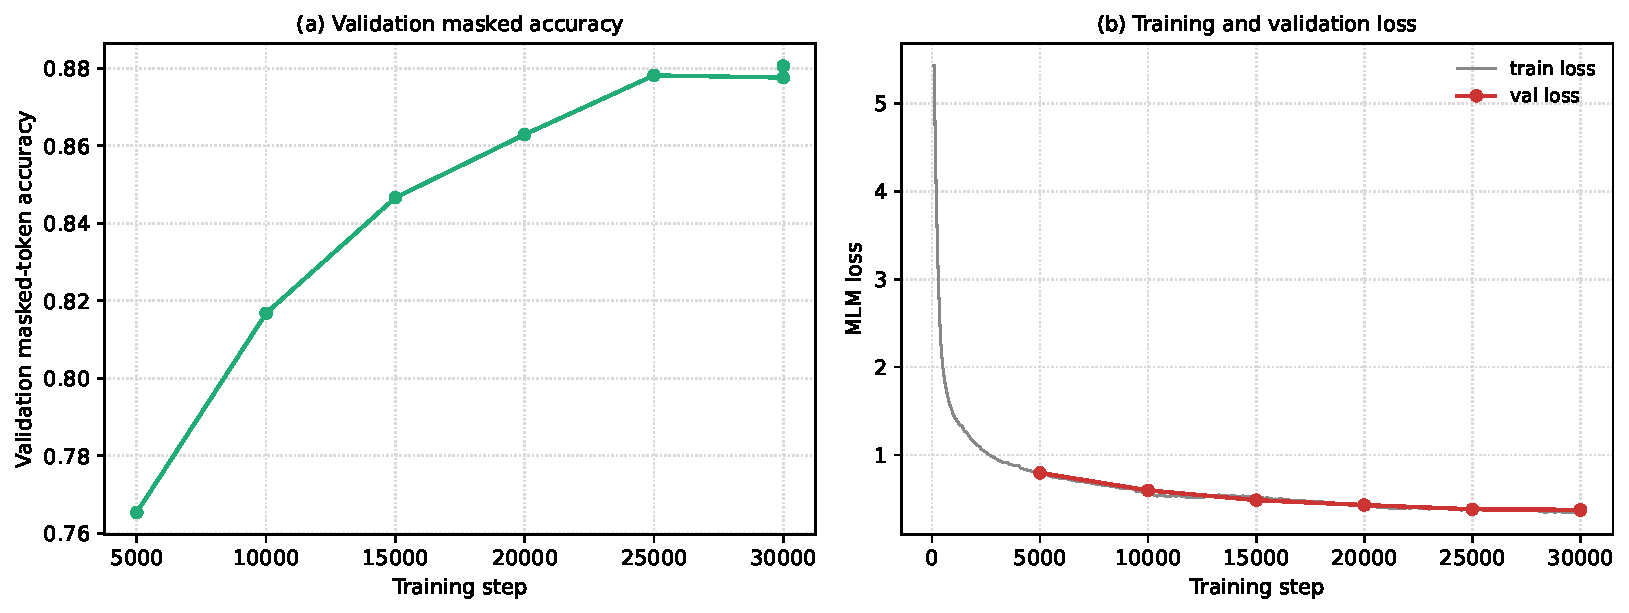
\includegraphics[width=\linewidth]{figures/Supplementary_2}
  \caption{%
    \textbf{Pretraining convergence of the released small \model{}.}
    Validation curves for the small model (standard masking,
    $4\!\times\!10^{-4}$) over 30{,}000 training steps.
    \textbf{(a)}~Validation masked-token accuracy.
    \textbf{(b)}~Training loss (dense) and validation MLM loss (markers).
    Both curves plateau smoothly, confirming stable convergence within the
    fixed 30{,}000-step budget. Per-step logs for the base model were not
    retained; its final validation metrics are reported in the sweep
    (\cref{fig:masking-sweep}).
  }%
  \label{fig:loss-curves}
\end{figure}

\FloatBarrier
\section{Tokeniser Details}%
\label{app:tokeniser}

% tables/tokenizer_table.tex
% SELFIES-adapted APE tokenizer statistics.
% All values from the tokenizer trained on 2M randomly sampled ChEMBL 36 SELFIES strings.
% Evaluated on 10,000 held-out ChEMBL 36 molecules.

\begin{table}[htbp]
  \centering
  \small
  \begin{tabular}{l r}
    \toprule
    \textbf{Tokenizer property} & \textbf{Value} \\
    \midrule
    \multicolumn{2}{l}{\textit{Vocabulary}} \\
    Training molecules          & \num{2000000} \\
    Base vocabulary (APE merges) & 589 \\
    Added \selfies{} primitives  & 42 \\
    Final vocabulary             & 631 \\
    \addlinespace
    \multicolumn{2}{l}{\textit{Sequence statistics (10\,000 held-out \chembl{}~36 molecules)}} \\
    Median length (tokens)       & 24 \\
    Mean length (tokens)         & 25.7 \\
    95th percentile              & 43 \\
    99th percentile              & 56 \\
    \addlinespace
    \multicolumn{2}{l}{\textit{Coverage}} \\
    Truncation at 128 tokens     & $<$0.1\% \\
    Unknown-token rate           & 0.0\% \\
    \bottomrule
  \end{tabular}
  \caption{%
    Summary statistics for the \selfies{}-adapted \ape{} tokenizer.
    The base vocabulary is learned by APE merge training on 2M randomly
    sampled \chembl{}~36 \selfies{} strings; 42 additional \selfies{} primitives
    observed in downstream benchmark molecules are appended after merge
    learning but before model pretraining, giving a final vocabulary of
    631 tokens on which all model weights are initialized and trained.
    Sequence statistics and coverage are evaluated on 10\,000 held-out
    \chembl{}~36 molecules.
  }%
  \label{tab:tokenizer-stats}
\end{table}


The final tokeniser is trained on 2M randomly sampled \chembl{}~36
\selfies{} strings with \texttt{max\_merge\_pieces\,=\,2} and
\texttt{min\_freq\_for\_merge\,=\,3000}, yielding a base vocabulary of
589 tokens.
An additional 42 \selfies{} primitives observed in the benchmark datasets
(minimum frequency $\ge 10$) are appended after \ape{} merge learning but
before model pretraining, giving a final vocabulary of 631 tokens on which
all model weights were initialised and trained from the outset.
Special tokens are assigned fixed ids: \texttt{[BOS]}\,=\,0,
\texttt{[PAD]}\,=\,1, \texttt{[EOS]}\,=\,2, \texttt{[UNK]}\,=\,3,
\texttt{[MASK]}\,=\,4.
Evaluated on 10\,000 held-out \chembl{}~36 molecules, the tokeniser
achieves an unknown-token rate of 0.0\%, a median sequence length of 24
tokens (mean 25.7; 95th percentile 43; 99th percentile 56), negligible
truncation at the model context length of 128 tokens ($<$0.1\%), and zero
truncations at 256 tokens.

\FloatBarrier
\section{Additional Benchmark Results}%
\label{app:additional-results}

This appendix reports per-task benchmark results, together with
auxiliary analyses used to assess robustness of the frozen-feature evaluation.
\Cref{tab:pertask} gives the full per-task test ROC-AUC for every model,
including the span- and heteroatom-span masking variants of \model{}-small.
Results not available for a given model--dataset combination are marked ``--'':
Tox21 for \model{}-base; HIV and MUV for the span-masking variant; and MUV,
SIDER, and Tox21 for the heteroatom-span variant.

{\footnotesize\setlength{\tabcolsep}{3.5pt}
\begin{longtable}{l r r r r r r r r }
  \toprule
  \textbf{Task} & \textbf{ECFP4} & \textbf{ChBa-2} & \textbf{SELF.} & \textbf{MoLF.} & \textbf{MMB-s} & \textbf{MMB-b} & \textbf{MMB-sp} & \textbf{MMB-h} \\
  \midrule
  \endfirsthead
  \toprule
  \textbf{Task} & \textbf{ECFP4} & \textbf{ChBa-2} & \textbf{SELF.} & \textbf{MoLF.} & \textbf{MMB-s} & \textbf{MMB-b} & \textbf{MMB-sp} & \textbf{MMB-h} \\
  \midrule
  \endhead
  \multicolumn{9}{l}{\textit{TDC -- ADME}} \\
  Bioavailability & 65.3 & 65.2 & 64.1 & 72.2 & 63.1 & 65.1 & 67.6 & 71.1 \\
  HIA & 93.9 & 88.7 & 88.4 & 98.1 & 97.8 & 98.0 & 98.1 & 97.9 \\
  Pgp & 91.6 & 84.3 & 83.3 & 92.9 & 91.5 & 93.0 & 90.6 & 92.0 \\
  PAMPA & 77.4 & 67.9 & 70.8 & 71.6 & 73.9 & 75.5 & 72.2 & 75.5 \\
  CYP1A2 & 91.9 & 87.6 & 86.5 & 91.4 & 90.4 & 91.3 & 89.9 & 90.9 \\
  CYP2C19 & 86.8 & 81.8 & 76.5 & 85.5 & 84.2 & 84.9 & 83.1 & 84.4 \\
  CYP2C9 & 86.7 & 82.1 & 80.5 & 86.6 & 84.9 & 84.9 & 84.6 & 85.3 \\
  CYP2D6 & 86.3 & 78.2 & 79.1 & 85.5 & 83.3 & 85.2 & 83.6 & 85.1 \\
  CYP3A4 & 86.3 & 80.5 & 78.7 & 85.0 & 83.1 & 83.6 & 81.9 & 83.3 \\
  CYP2C9 (substrate) & 62.1 & 65.6 & 60.4 & 62.5 & 62.0 & 62.6 & 60.7 & 59.4 \\
  CYP2D6 (substrate) & 79.0 & 78.7 & 71.4 & 83.0 & 79.2 & 82.0 & 78.8 & 78.8 \\
  CYP3A4 (substrate) & 65.4 & 67.2 & 61.2 & 63.1 & 62.1 & 62.4 & 65.0 & 66.9 \\
  \addlinespace
  \multicolumn{9}{l}{\textit{TDC -- Toxicity}} \\
  AMES & 84.7 & 74.7 & 70.5 & 81.7 & 78.3 & 78.2 & 78.2 & 78.2 \\
  DILI & 88.2 & 73.9 & 74.3 & 92.0 & 92.3 & 89.3 & 93.2 & 90.2 \\
  hERG & 80.2 & 64.3 & 79.1 & 83.1 & 81.6 & 84.9 & 80.5 & 80.2 \\
  hERG (Karim) & 87.1 & 79.5 & 74.5 & 84.1 & 82.4 & 82.8 & 81.4 & 82.2 \\
  \addlinespace
  \multicolumn{9}{l}{\textit{TDC -- HTS}} \\
  SARS-CoV-2 3CLPro & 76.1 & 67.6 & 66.6 & 74.9 & 70.7 & 73.2 & 73.0 & 71.9 \\
  SARS-CoV-2 (Vitro) & 61.0 & 64.9 & 55.7 & 58.7 & 58.9 & 55.6 & 54.6 & 56.5 \\
  \addlinespace
  \multicolumn{9}{l}{\textit{MoleculeNet}} \\
  BACE & 86.2 & 80.8 & 78.4 & 83.7 & 78.4 & 81.5 & 78.6 & 80.1 \\
  BBBP & 70.2 & 70.7 & 65.4 & 71.5 & 69.3 & 68.3 & 69.3 & 68.3 \\
  ClinTox & 73.1 & 55.9 & 79.0 & 88.4 & 79.2 & 82.1 & 81.6 & 83.2 \\
  HIV & 78.4 & 75.3 & 75.9 & 78.0 & 76.2 & 73.3 & -- & 75.5 \\
  MUV & 72.4 & 56.6 & 57.7 & 79.8 & 70.5 & 54.7 & -- & -- \\
  SIDER & 67.4 & 61.6 & 56.6 & 66.6 & 64.7 & 64.3 & 63.5 & -- \\
  Tox21 & 75.9 & 69.4 & 69.0 & 75.0 & 73.9 & -- & 73.6 & -- \\
  \addlinespace
  \bottomrule
  \caption{Per-task test ROC-AUC ($\times100$) for all models on the 25-task benchmark. \emph{MMB-s} = \model{}-small (standard), \emph{MMB-b} = \model{}-base, \emph{MMB-sp} = small span masking, \emph{MMB-h} = small hetero-span masking. ``--'' marks evaluations not yet run.}\label{tab:pertask}
\end{longtable}
}


\begin{table}[htbp]
  \centering\small
  \begin{tabular}{l l r r r r r r}
    \toprule
    \textbf{Model A} & \textbf{Model B} & \textbf{$n$} & \textbf{Wins} & \textbf{Ties} & \textbf{Losses} & \textbf{Mean $\Delta$} & \textbf{95\,\% CI} \\
    \midrule
    MMB-base & SELFormer & 25 & 23 & 0 & 2 & +5.79 & $[+4.2,\;+7.5]$ \\
    MMB-base & ChemBERTa-2 & 25 & 19 & 0 & 6 & +5.00 & $[+2.1,\;+8.1]$ \\
    MMB-base & ECFP4 & 25 & 7 & 0 & 18 & -1.02 & $[-2.3,\;+0.4]$ \\
    MMB-base & MoLFormer & 25 & 4 & 0 & 21 & -1.87 & $[-2.9,\;-0.9]$ \\
    \bottomrule
  \end{tabular}
  \caption{%
    Paired bootstrap confidence intervals (95\,\%, $B=10{,}000$ resamples) on
    mean $\Delta$ ROC-AUC ($\times100$) between \model{}-base and each baseline,
    computed over the tasks where both models have a result.
    \emph{Wins}/\emph{Ties}/\emph{Losses} count tasks where \model{}-base is
    above, equal to, or below the baseline.
    A positive mean $\Delta$ and CI entirely above zero indicates a consistent
    advantage for \model{}-base.
  }%
  \label{tab:bootstrap-cis}
\end{table}


\begin{figure}[htbp]
  \centering
  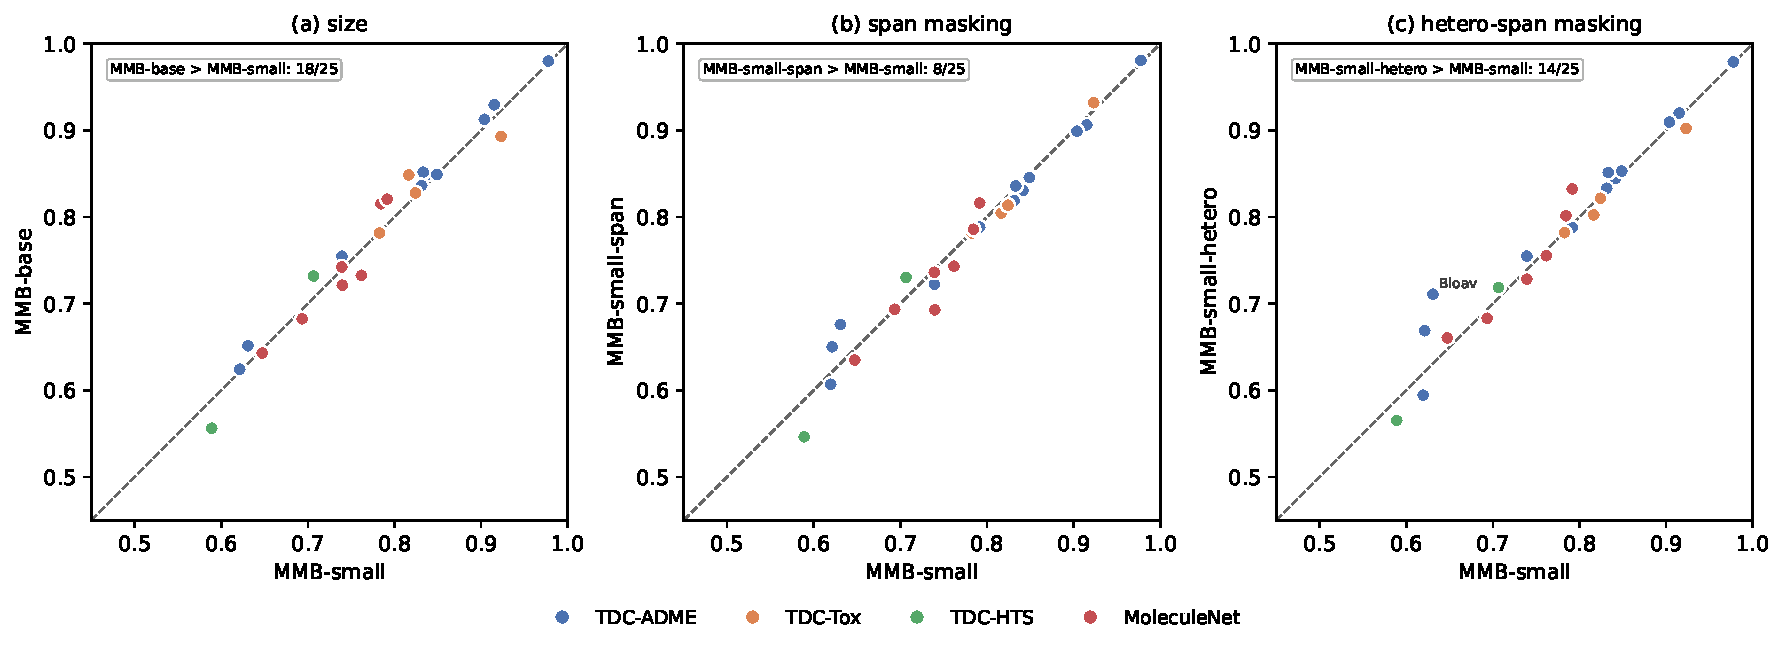
\includegraphics[width=\linewidth]{figures/Fig_2}
  \caption{%
    \textbf{Internal comparison of the four \model{} checkpoints on downstream
    ROC-AUC.}
    Paired scatter of held-out test ROC-AUC across the benchmark tasks (one
    point per task, best cross-validated downstream head), isolating each
    pretraining design axis against the released small model (standard masking,
    $y$-axis throughout except panel a).
    \textbf{(a)}~\model{}-small versus \model{}-base, isolating model size.
    \textbf{(b)}~\model{}-small versus the span-masking variant.
    \textbf{(c)}~\model{}-small versus the heteroatom-biased span-masking
    variant. The dashed line is the identity $y=x$, points are coloured by task
    group, and each inset reports the number of tasks on which the $y$-axis
    model wins. Panel a is evaluated on 24 jointly evaluated datasets
    (\model{}-base lacks Tox21) and panels b and c only on the tasks available
    for the respective variant (23 and 22 of 25; see \cref{tab:pertask}).
  }%
  \label{fig:four-model}
\end{figure}

\FloatBarrier
\section{Molecular Embedding Models}%
\label{app:embedders}

\Cref{tab:embedders-full} lists the non-graph molecular embedding
models evaluated in the benchmark of
\citet{praskiBenchmarkingPretrainedMolecular2025}.
Graph-based models (R-MAT, MAT, GROVER, GIN, MolR, GraphMVP,
Uni-Mol, Uni-Mol2, GEM, GraphFP) are excluded here as they fall
outside the scope of \model{}.
Table~6 of \citet{praskiBenchmarkingPretrainedMolecular2025} provides
the full benchmark results across all 25 methods, including graph-based
architectures.

\input{tables/embedders_table}

\FloatBarrier
\section{Pretraining Hyperparameter Heatmaps}%
\label{app:masking-heatmaps}

This appendix reports the full hyperparameter sweep underlying the masking and
learning-rate selections discussed in \cref{sec:ablations}, as heatmaps over all
masking probabilities, strategies, and learning rates evaluated.

\begin{figure}[H]
  \centering
  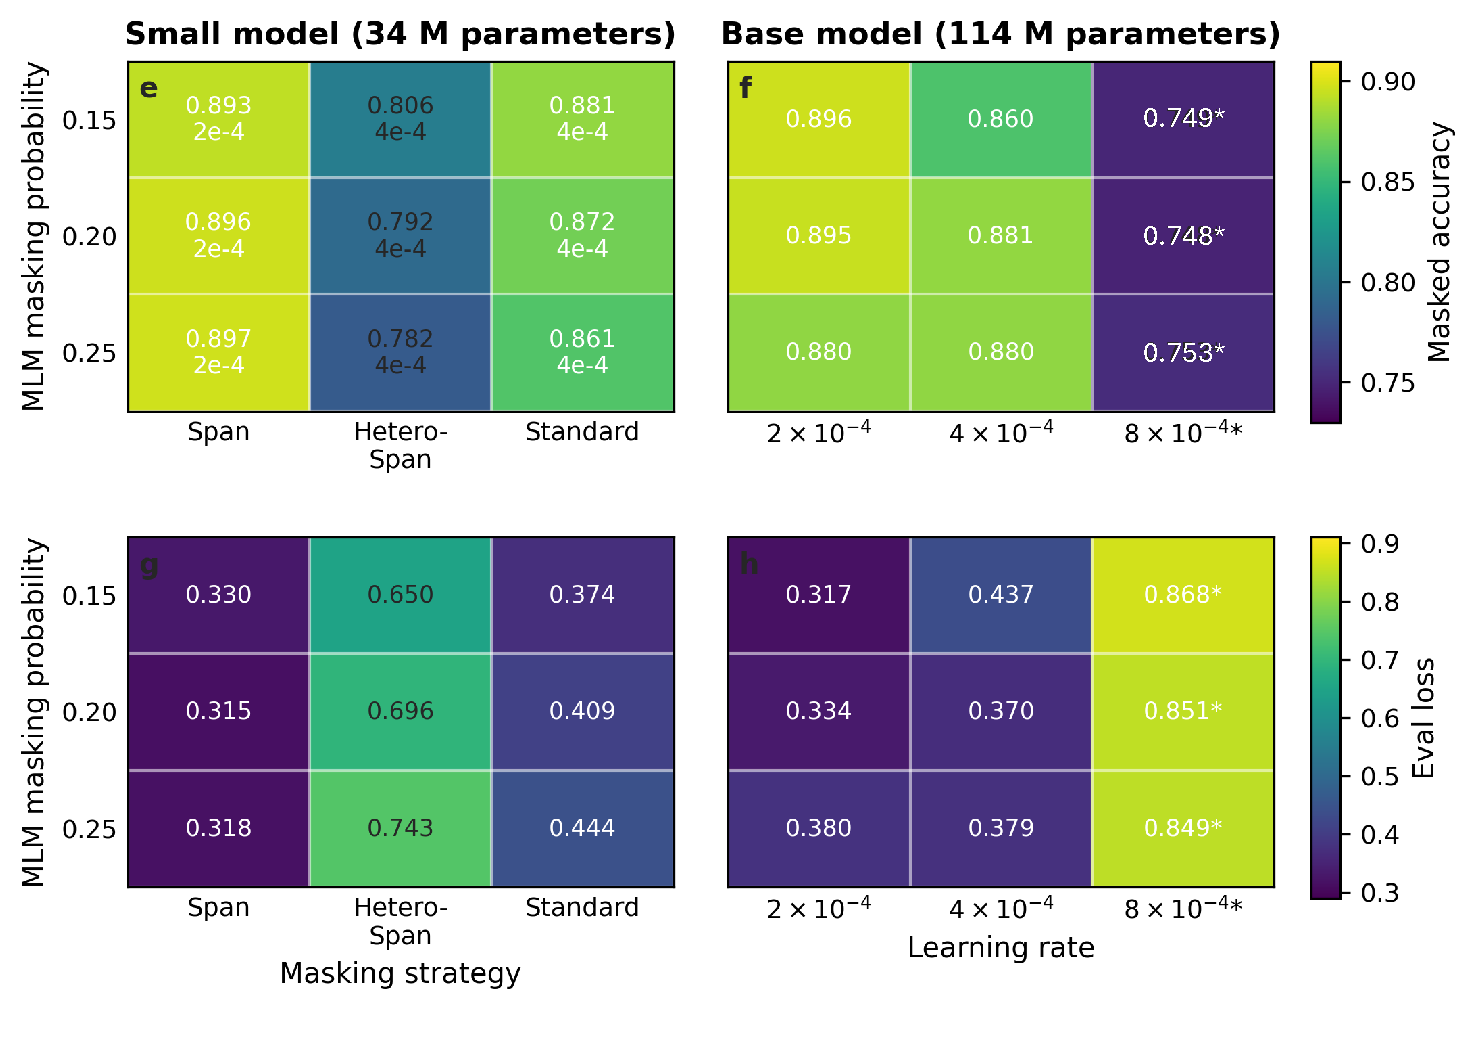
\includegraphics[width=\linewidth]{figures/Supplementary_1}
  \caption{%
    \textbf{Masked language modelling sweep across masking strategies,
    masking probabilities, and learning rates.}
    Heatmaps show validation performance for the small \model{} model
    ($\sim$34\,M parameters) and the base \model{} model ($\sim$114\,M
    parameters).
    Panels \textbf{e} and \textbf{f} show masked-token accuracy
    (higher is better).
    Panels \textbf{g} and \textbf{h} show evaluation loss (lower is better).
    For the small model, columns compare masking strategies: span masking,
    hetero-span masking, and standard token masking.
    For the base model, columns compare peak learning rates under standard
    masking: $2\!\times\!10^{-4}$, $4\!\times\!10^{-4}$,
    and $8\!\times\!10^{-4}$.
    Rows give the MLM masking probability: 0.15, 0.20, and 0.25.
    For the small model, the second line in each cell reports the learning
    rate used; asterisks denote runs that diverged during training.
    On validation MLM metrics, the small model performs best with span
    masking at a learning rate of $2\!\times\!10^{-4}$, with accuracy
    increasing slightly as masking probability increases.
    Hetero-span masking is consistently worse for both accuracy and loss.
    For the base model, $2\!\times\!10^{-4}$ and $4\!\times\!10^{-4}$
    perform similarly; $8\!\times\!10^{-4}$ produces unstable training
    with superficially moderate final accuracy but elevated loss.
    Line-plot views of panels a--d are shown in the main text
    (\cref{fig:masking-sweep}).
  }%
  \label{fig:masking-heatmap}
\end{figure}

\end{appendices}

\end{document}
